\documentclass[14pt,a4paper]{article} %openany
\usepackage[affil-it]{authblk}
\usepackage[english]{babel}
\usepackage{graphicx}
\usepackage{rotating}
%\usepackage{bibtex}
%\usepackage[utf8]{inputenc}
%\usepackage[english]{babel}
\usepackage{adjustbox}
\usepackage{courier}
\usepackage{verbatim}
\usepackage{url}
\usepackage{float}
\usepackage{array}
\usepackage{breakcites}
\usepackage{gensymb}
%\usepackage[backend=biber]{biblatex}
\usepackage{booktabs,tabularx}
\usepackage{listings}
\usepackage{appendix}
\usepackage{cite}
\usepackage{blindtext}
\usepackage[utf8]{inputenc} % Required for inputting international characters
\usepackage[T1]{fontenc} % Output font encoding for international characters
\usepackage{mathpazo} % Palatino font
\usepackage{graphicx} % For the logo
\usepackage{hyperref}
\hypersetup{
    colorlinks=true,
    linkcolor=blue,
    filecolor=magenta,      
    urlcolor=cyan,
}
 
\urlstyle{same}
 
%\bibliographystyle{numeric}

\begin{document}

%----------------------------------------------------------------------------------------
%    TITLE PAGE
%----------------------------------------------------------------------------------------

\begin{titlepage} % Suppresses displaying the page number on the title page and the subsequent page counts as page 1
    \newcommand{\HRule}{\rule{\linewidth}{0.5mm}} % Defines a new command for horizontal lines, change thickness here
    
    \center % Centre everything on the page

    %------------------------------------------------
    %    Title
    %------------------------------------------------
    
    \HRule\\[0.2cm]
    
     \begin{minipage}{0.4\textwidth}
        
\includegraphics[width=\textwidth]{arfc-logo}
        \end{minipage}%
        \begin{minipage}{0.6\textwidth}
        {\begin{flushright}\huge\bfseries Dynamic Transition Analysis With TIMES\end{flushright}}
        {\begin{flushright}\large\textit{I\textsuperscript{2}CNER Project Report}\end{flushright}}

        \end{minipage}

    \vspace{0.2cm}
    \HRule
    \vspace{0.5cm}
    
    %------------------------------------------------
    %    Author(s)
    %------------------------------------------------
    
    \begin{minipage}{0.4\textwidth}
        \begin{flushleft}
            \large
            \textit{Author}\\
            Huan \textsc{Yan}\\
        \end{flushleft}
    \end{minipage}
    ~
    \begin{minipage}{0.4\textwidth}
        \begin{flushright}
            \large
            \textit{Principal Investigator}\\
            Kathryn D. \textsc{Huff} % Supervisor's name
        \end{flushright}
    \end{minipage}
    
    % If you don't want a supervisor, uncomment the two lines below and comment the code above
    %{\large\textit{Author}}\\
    %John \textsc{Smith} % Your name

    %------------------------------------------------
    %    Report Number
    %------------------------------------------------
    \vspace{1cm}
    \textsc{\LARGE\bfseries UIUC-ARFC-2019-09} \textit{work in progress} % Replace YYYY with the year, NN with report index
    \vspace{0.5cm}
    
    %------------------------------------------------
    %    Date
    %------------------------------------------------
    
    \vspace{0.5cm} % Position the date further down the remaining page
    {\large\today} % Date, change the \today to a set date if you want to be precise
    \vspace{0.5cm}

%------------------------------------------------
    %    Headings
    %------------------------------------------------
    
    \textsc{\LARGE Advanced Reactors and Fuel Cycles}\\[0.25cm] % Research Group
    
    \textsc{\large Dept. of Nuclear, Plasma, \& Radiological Engineering}\\% Department
    
    \textsc{\large University of Illiois at Urbana-Champaign}\\ % University


    
    %------------------------------------------------
    %    Logo
    %------------------------------------------------
    
    
    \vspace{0.5cm}
    
\includegraphics[scale=0.2]{arfc-logo}
    
\includegraphics[scale=0.3]{i2cner_logo}
    
\includegraphics[scale=0.2]{wpi_logo}
    
\includegraphics[scale=0.04]{ku_logo}\\[1cm] % Include a department/university logo - this will require the graphicx package
     
    %----------------------------------------------------------------------------------------

    %------------------------------------------------
    %   Funding 
    %------------------------------------------------
    % For this section, either use \vfill to fill the space 
    % or insert funding acknowledgement
    \textit{The authors gratefully acknowledge the support of the International Institute for Carbon
Neutral Energy Research (WPI-I2CNER), sponsored by the Japanese Ministry of Education, Culture, Sports, Science and Technology.}  

\end{titlepage}

\section{Introduction}
This report summarizes the summer working progress made on TIMES model for Japan energy transition analysis, including major model changes that facilitates the analysis of the impact of I$^2$CNER technology.

\section{Progress Summary}
\subsection{Availability Factors of Renewable Energy}
TIMES analysis framework allows users to explicitly define the availability factor of processes in each time invervals. With this function, the intermittent feature of renewable energy can be modeled in a relistic way. In this model, solar and wind power are two major intermittent power generation processes considered.\\
There are four time levels in TIMES framework and currently in this model we consider "Annual" and "Daynite", with the later can be arbitrarily divided. To model the availability of solar and wind energy, time-slices where each process is available are created and the availability factors are defined close to 1, while in other time-slices this value is zero. The hierarchy of the time-slices used in this model is shown in Figure \ref{fig:time}. The length of each time-slices is calculated based on the average sunshine duration in Japan and also inferred from the availability factor of wind power. It is assumed that the availability of these two processes are independent. 
The purpose of explicitly modeling availability factor in each time-slice is to enforce the backup power deployment for renewable energy. In reality the supply from solar and wind power is intermittent while the demand is not, large capacity of backup power or energy storage is required to fully exploit the benefit of renewable energy.

\begin{figure}[H]
  \centering
    \includegraphics[width=1\textwidth]{./plot/timeslices.jpg}
  \caption{Hierarchical structure of time slices and corresponding duration }
  \label{fig:time}
\end{figure}

\subsection{Time-dependent Power Demand}
The power demand is strongly time-dependent. Usually the demand is higher in the daytime and summer. It could affect the deployment of energy storage device considering the availability of solar energy follows the similar pattern. So it would be beneficial to make the demand in each time-slice follow a realistic pattern. The time-dependent power demand is enabled after 2017. The percentage of power demand for each period is shown in Figure.\ref{fig:demand}.

\begin{figure}[H]
  \centering
    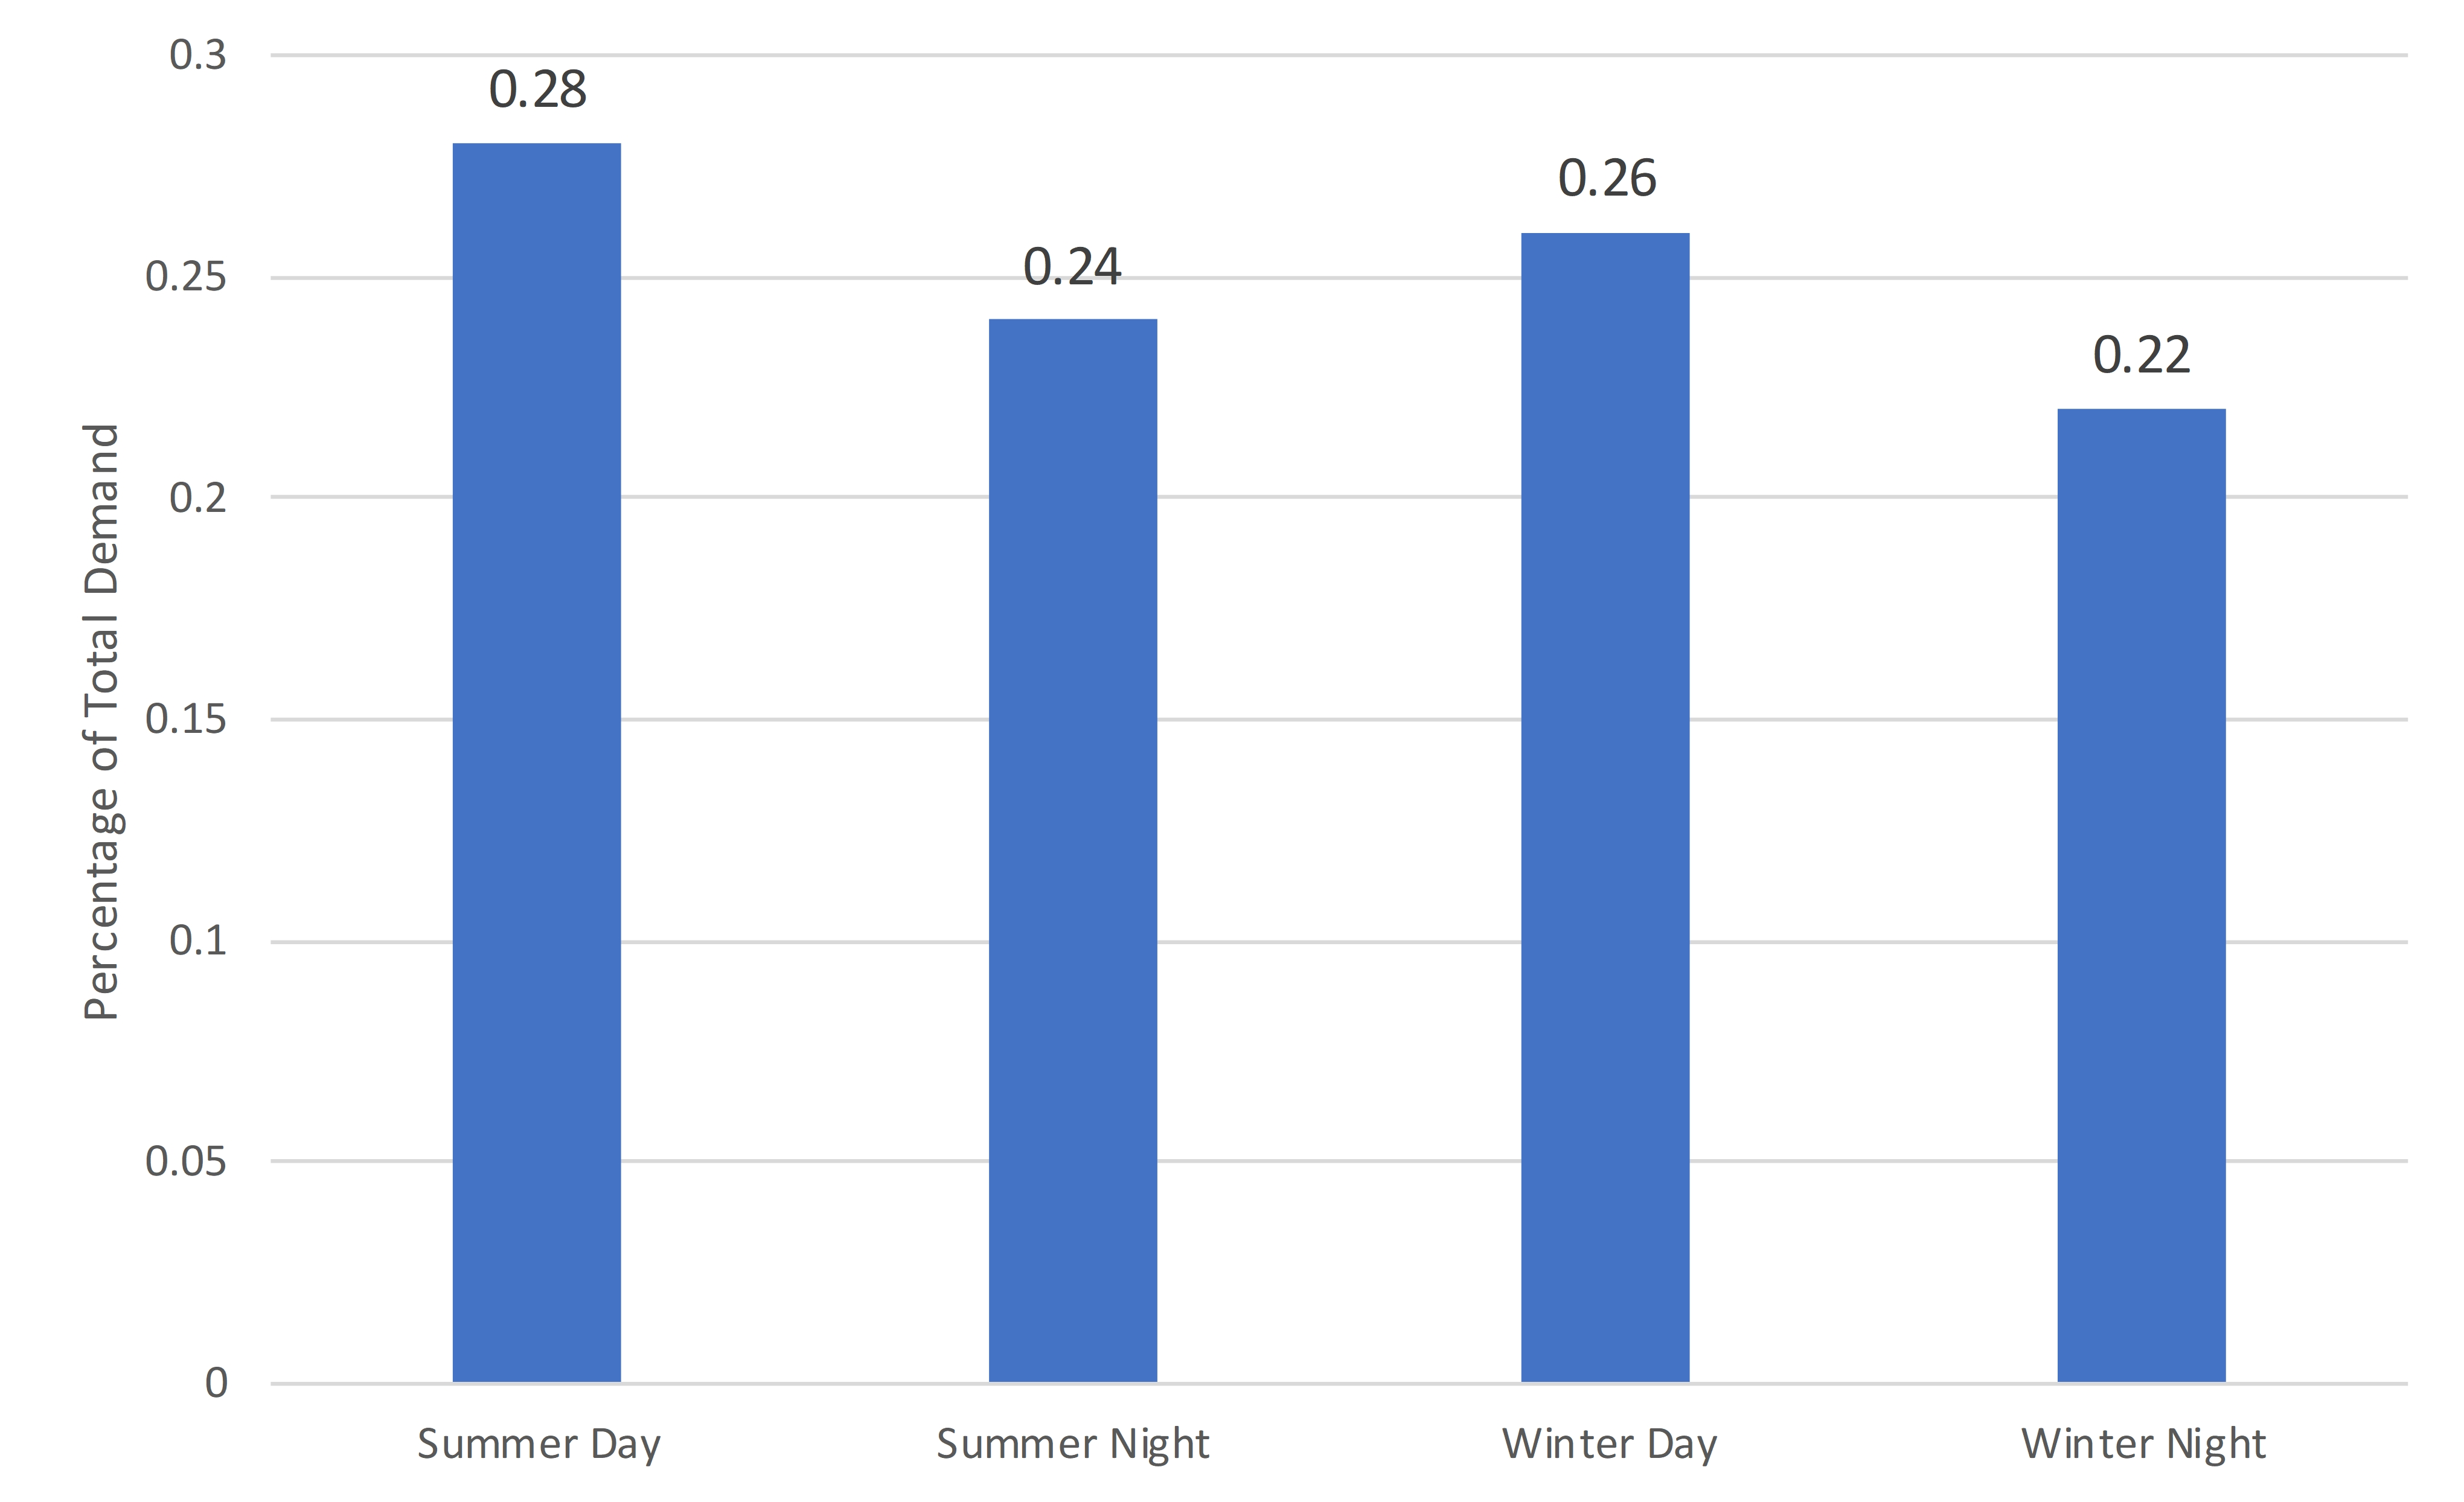
\includegraphics[width=0.8\textwidth]{./plot/demand.jpg}
  \caption{Percentage of total demand by time periods.}
  \label{fig:demand}
\end{figure}

\subsection{Hydrogen Economy}
To model the effect of development of hydrogen economy, it is required to explicitly consider the cost of different types of fuel. In the current model only two processes involving natural gas and oil are restructured to include fuel cost. Nominal prices of natural gas and oil are assumed and added to the corresponding importing processes. And these costs are removed from the variable costs of all processes that consume natural gas and oil.

\subsubsection{Refinery Process}
Modeling hydrogen production is the first step of modeling the hydrogen economy. Currently the hydrogen mass production is through steam reforming of natural gas. This process results in net reduction of energy and is reflected in efficiency\cite{sheet2005hydrogen}. Note that two types of steam reforming are considered, either with or without CCS. We assumed that without CCS the carbon emission is equivalent to directly using natural gas in electricity production. CCS steam reforming is available after 2030 and the emission is reduced to zero. Note that for simplicity only the fuel cost is considered in the hydrogen production process.
Besides steam reforming, electrolysis and photocatalysis are also considered as alternative for hydrogen production. Electrolysis is modeled as transforming electricity to hydrogen with some lost of energy and zero emission. There are different electrolysis technologies with different efficiency around 80\%\cite{ursua2011hydrogen}. In current model only one electrolysis process with 80\% efficiency is included.
Photocatalysis is an alternative hydrogen production technology that currently under development and is a part fof I$^2$CNER research portfolio. This technology is envisioned as directly using sunlight to split water, as opposed to PV and electrolysis system. In the model this process is modeled in a similar fashion as solar power, with the same definition of availability factor. Currently in the model the cost data associated with photocatalysis is taken from \cite{pinaud2013technical} as variable cost for unit production of hydrogen.
Also, as stated in the following section, to model the transportation sector which requires different types of fuel, the crude oil refinery is also included. Currently the process is directly borrowed from the VEDA demo model and only gasoline is used. We can further include process such as residential heating or diesel car to use other fuels. Or the extra fuels can be handled by export process to bring down the overall system costs.

\subsubsection{Modeling Transportation Sector}
It is recognized that a major part of I$^2$NER technology contributions is through hydrogen economy. Shifting to hydrogen as energy carrier will have significant impact on transportation sector. In fact, according to the technology roadmap published by Ministry of Economy, Trade and Industry, Japan plans to achieve 800,000 hydrogen fuel cell vehicles on road by 2030, with technology advances bring the cost and performance of FCV to the level that rivals conventional vehicle\cite{japan_fc_roadmap}. It is reasonable to model the demand from transportation sectors to see if the results align with the roadmap.
Currently only passenger transportation is modeled. However the freight transportation also accounts for a large part of carbon emission so it needs to be included as well.
The demand for passenger transportation is expressed in the unit of KPassenger*KM/Year and the data is from OECD database\cite{oecd}. Since the population of Japan is unlike to increase in the future it is assumed that the demand will stay constant. For personal sector, only three types of vehicle are considered: traditional gasoline car, electric car and hydrogen fuel cell car. The efficiency can be inferred from fuel economy data. The availability of each vehicle is expressed in the mileage traveled per year. The parameters are summarized in Table.\ref{tab:car}. Compared to electric vehicle, with easier refueling procedures the hydrogen and gasoline car can travel longer distances per year. Due to the technology advance and increased production of fuel cell, it is assumed that the performance and price of electric car and hydrogen car will be brought down to the same level as conventional gasoline car by 2030. Note that in order to preserve the initial conditions the modeling of transportation sector starts from 2017 rather than 2013.

\begin{table}[htbp]
\small
\setlength\tabcolsep{0.1pt}
\centering
\begin{tabular}{|c|c|c|c|c|c|c|}
\hline
\begin{tabular}[c]{@{}c@{}}Vehicle\\  Type\end{tabular} & \begin{tabular}[c]{@{}c@{}}Mileage \\ (km/year)\end{tabular} & \begin{tabular}[c]{@{}c@{}}Passenger\\ /Car\end{tabular} & \begin{tabular}[c]{@{}c@{}}Investment\\  Cost (\$)\end{tabular} & \begin{tabular}[c]{@{}c@{}}Maintenance\\  Cost \\ (\$/year)\end{tabular} & \begin{tabular}[c]{@{}c@{}}Life \\ (year)\end{tabular} & \begin{tabular}[c]{@{}c@{}}Efficiency\\  (MV*km/GWh)\end{tabular} \\ \hline
Gasoline & 12000 & 1.25 & 15500 & 150 & 10 & 1.152 \\ \hline
Electric & 8000 & 1.25 & 20000 & 150 & 10 & 4.548 \\ \hline
\begin{tabular}[c]{@{}c@{}}Hydrogen\\  Fuel Cell\end{tabular} & 12000 & 1.25 & 70000 & 150 & 10 & 5.776 \\ \hline
\end{tabular}
\caption{Personal vehicle parameters.}
\label{tab:car}
\end{table}


\subsection{Storage Process}
Energy storage is a crucial part of power grid due to the intermittent feature of some renewable energy. In current model two storage processes were added to account for the storage of electricity and hydrogen. The capacity of storage process corresponds to the charging rate of the process while the activity corresponds to the amount of energy it can store. The later can be specified using CAP2ACT.
Currently only one type of battery with total storage capacity of 8GWh per GW was added to the model.The efficiency is assumed to be 80\% (20\% of electricity loss from charging-discharging). The estimated cost for battery from EIA is used\cite{outlook2019technical}. This device can be replaced if detailed data are available.
Hydrogen can be stored in specialized high pressure gas tanks. The cost of storage is inferred from the estimated hydrogen storage volume and pressure of such device\cite{james2016hydrogen}.

\subsection{Refining Model Constraints}

\subsubsection{Growth Rate of Capacity}
In the previous model there's no constraint on the growth rate of capacity except for those explicitly defined lumpy investments. However, in reality the increment of new capacity is limited. Without such limit, the model will deploy renewable energy in a unrealistic pace. In current model it is assumed that new capacity (including vehicles) can only grow by 30\% each year. It might be more appropriate to limit the absolute amount of new capacity each year but TIMES doesn't offer a simple way to implement such constraint.
.
\subsubsection{CO2 Emission Constraint}
In the previous model, the CO$_2$ emission limit is linearly interpolated between the current emission and the objective of the final year.
However, after implementation of the growth rate constraint on the new capacity, the model will be infeasible due to the slower deployment of renewable energy and increasing power demand. It is realized that due to the assumption of increasing demand we have to allow for a period of time where emission increases relative to base year level. The detailed analysis will be shown in the following section.

\subsubsection{Constraint on Wind Power Capacity}
The constraint on the max capacity of wind power is replaced by the estimation of the theoretical max capacity in Japan. \cite{heger_wind_2016}


\section{Results}

In this part some results generated by current model will be presented. Two scenarios, with and without new nuclear reactors, are compared. Note that the new installment of reactors is limited to one reactor per year.

\subsection{Capacity and Power Output}
The installed capacity for the two scenarios are shown in Figure.\ref{fig:nonuccap} and Figure.\ref{fig:nuccap}. The exclusion of new nuclear reactor clearly encourages significantly more installation of renewable energy and earlier introduction of hydrogen fuel cell as a main electricity production method. As revealed in section \ref{sec:hydrogen production}, the deployment of hydrogen fuel cells relies on the highly efficient photocatalytic hydrogen production method. Other pathways, such as PV plus electrolysis, are rejected by model probably due to higher cost and lower system efficiency. Interestingly, the model suggests no need for direct electricity storage, except tiny amount of battery installed near 2100. Most energy will be stored in the form of hydrogen (See section \ref{sec:hydrogen production}). 
\begin{figure}[H]
  \centering
    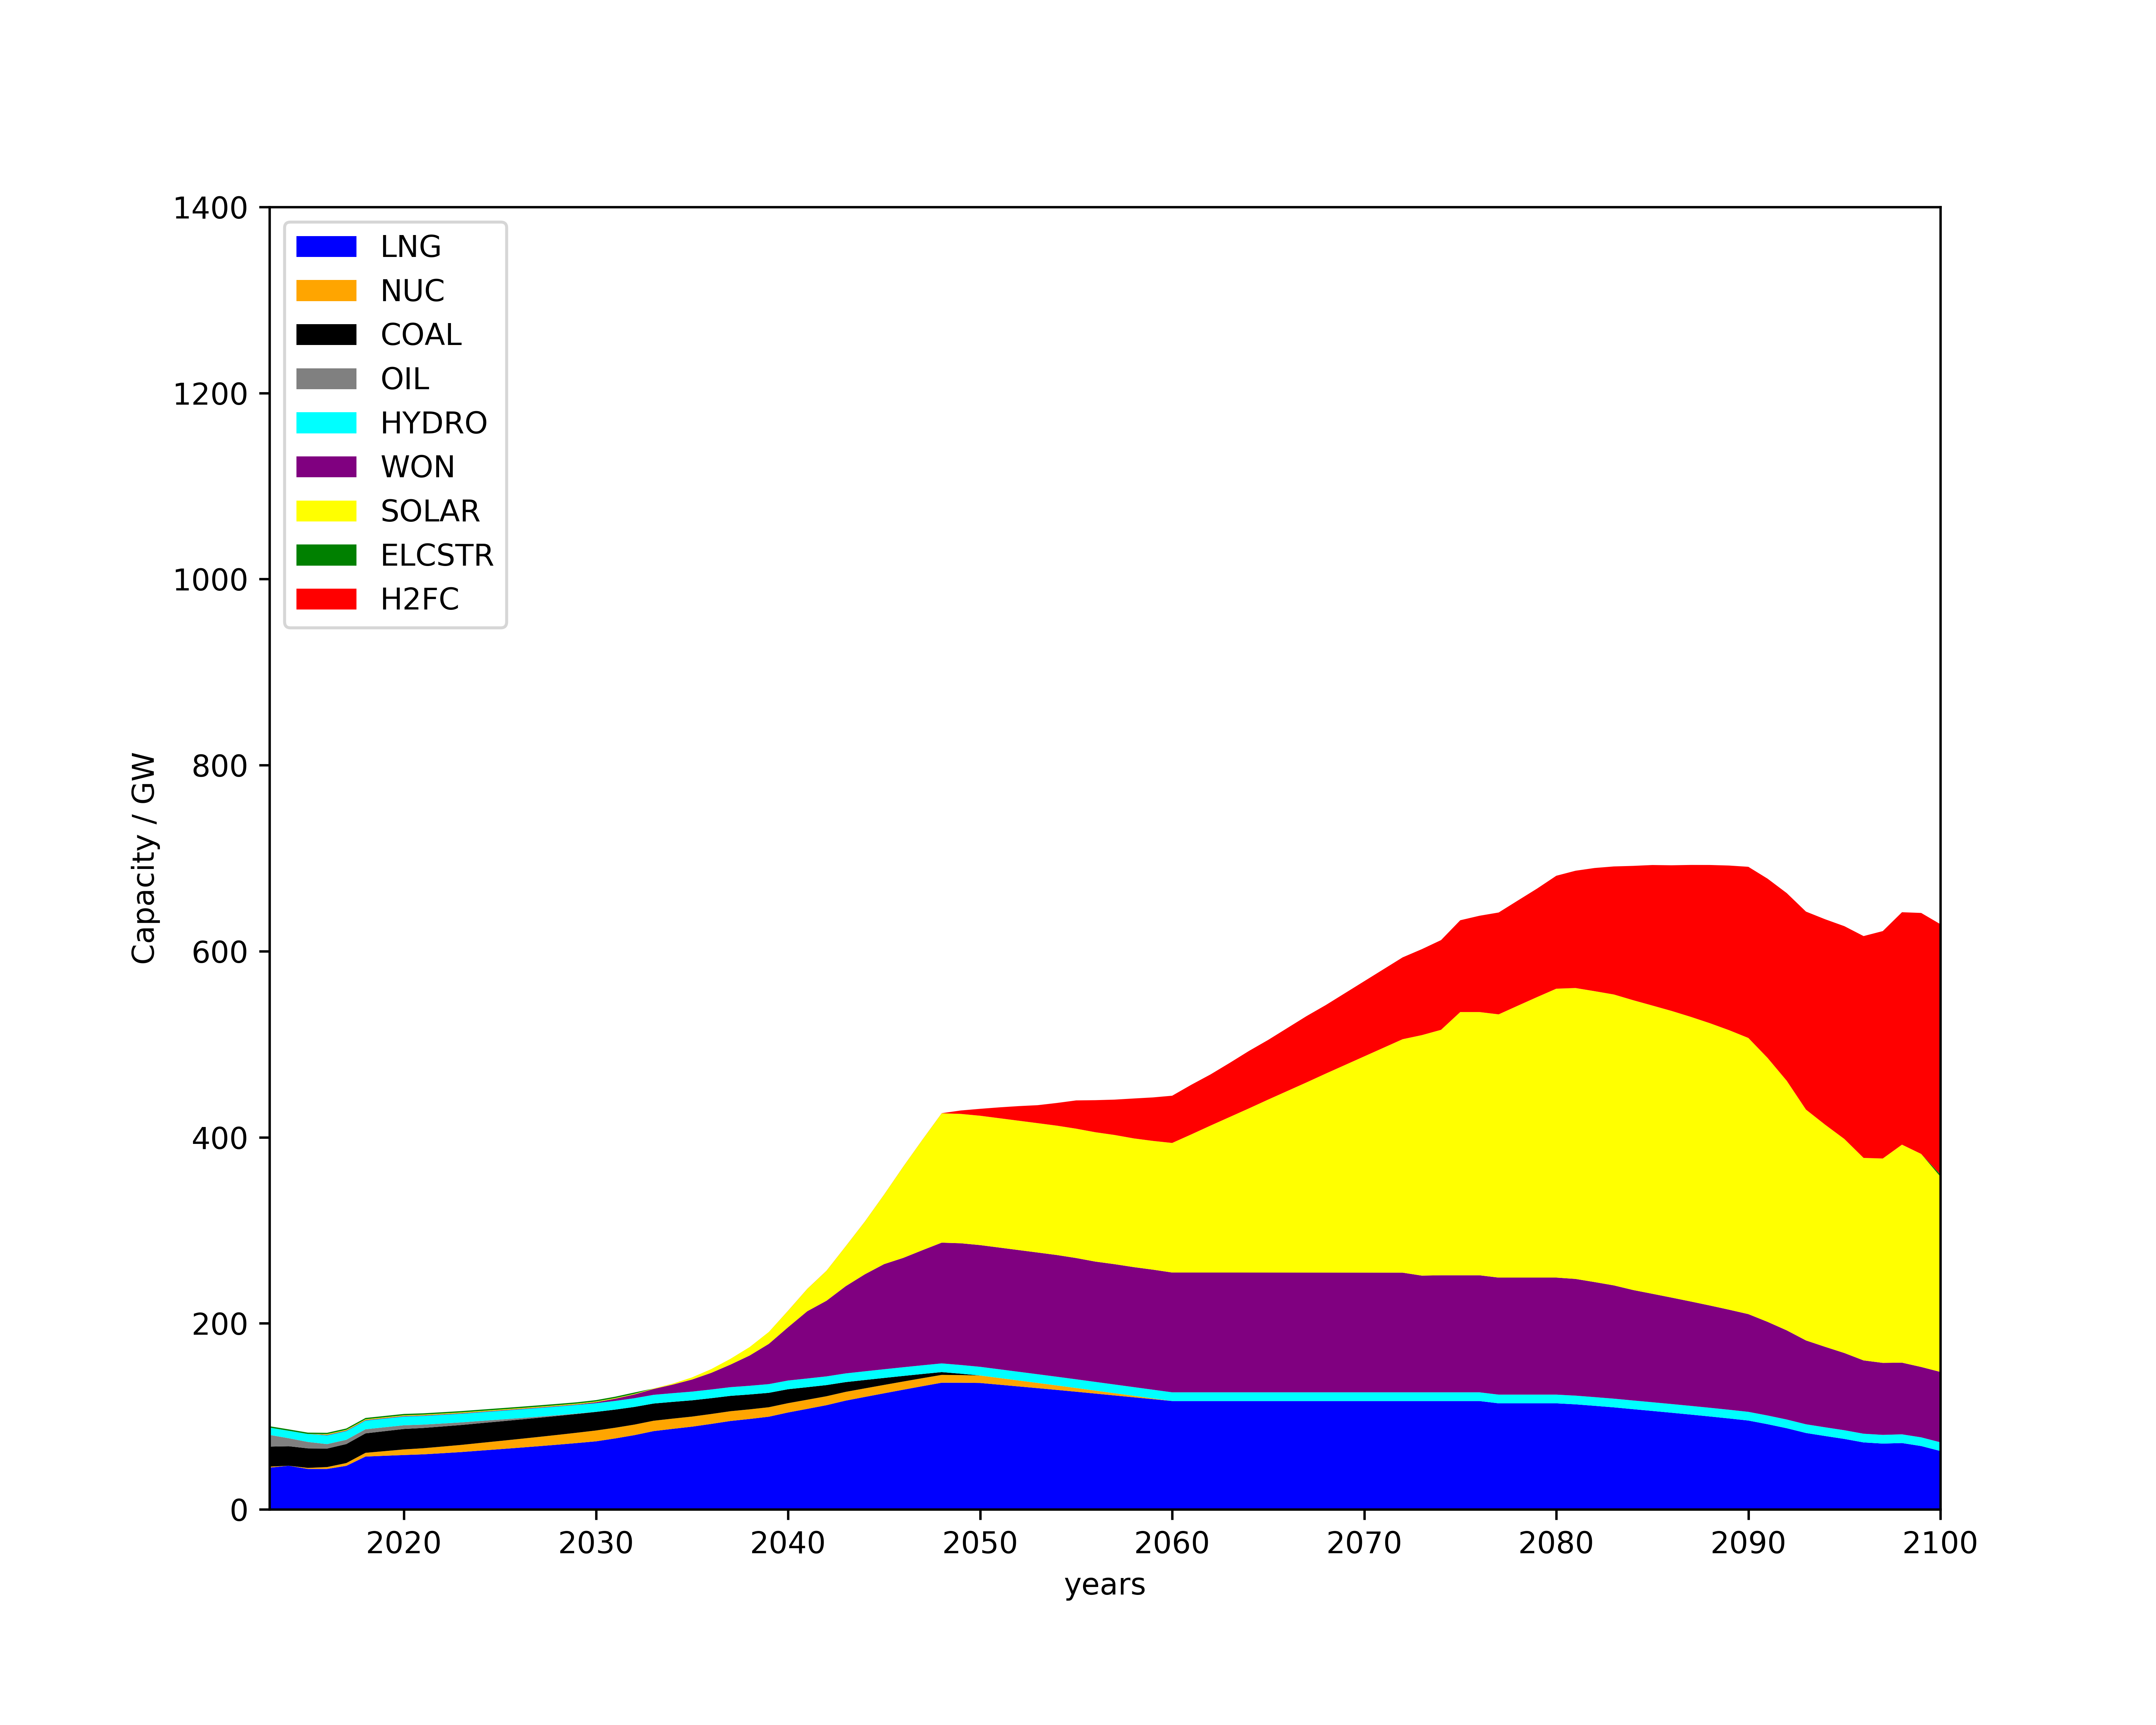
\includegraphics[width=0.9\textwidth]{./plot/nonuc_cap.png}
  \caption{Installed capacity without new reactors.}
  \label{fig:nonuccap}
\end{figure}
\begin{figure}[H]
  \centering
    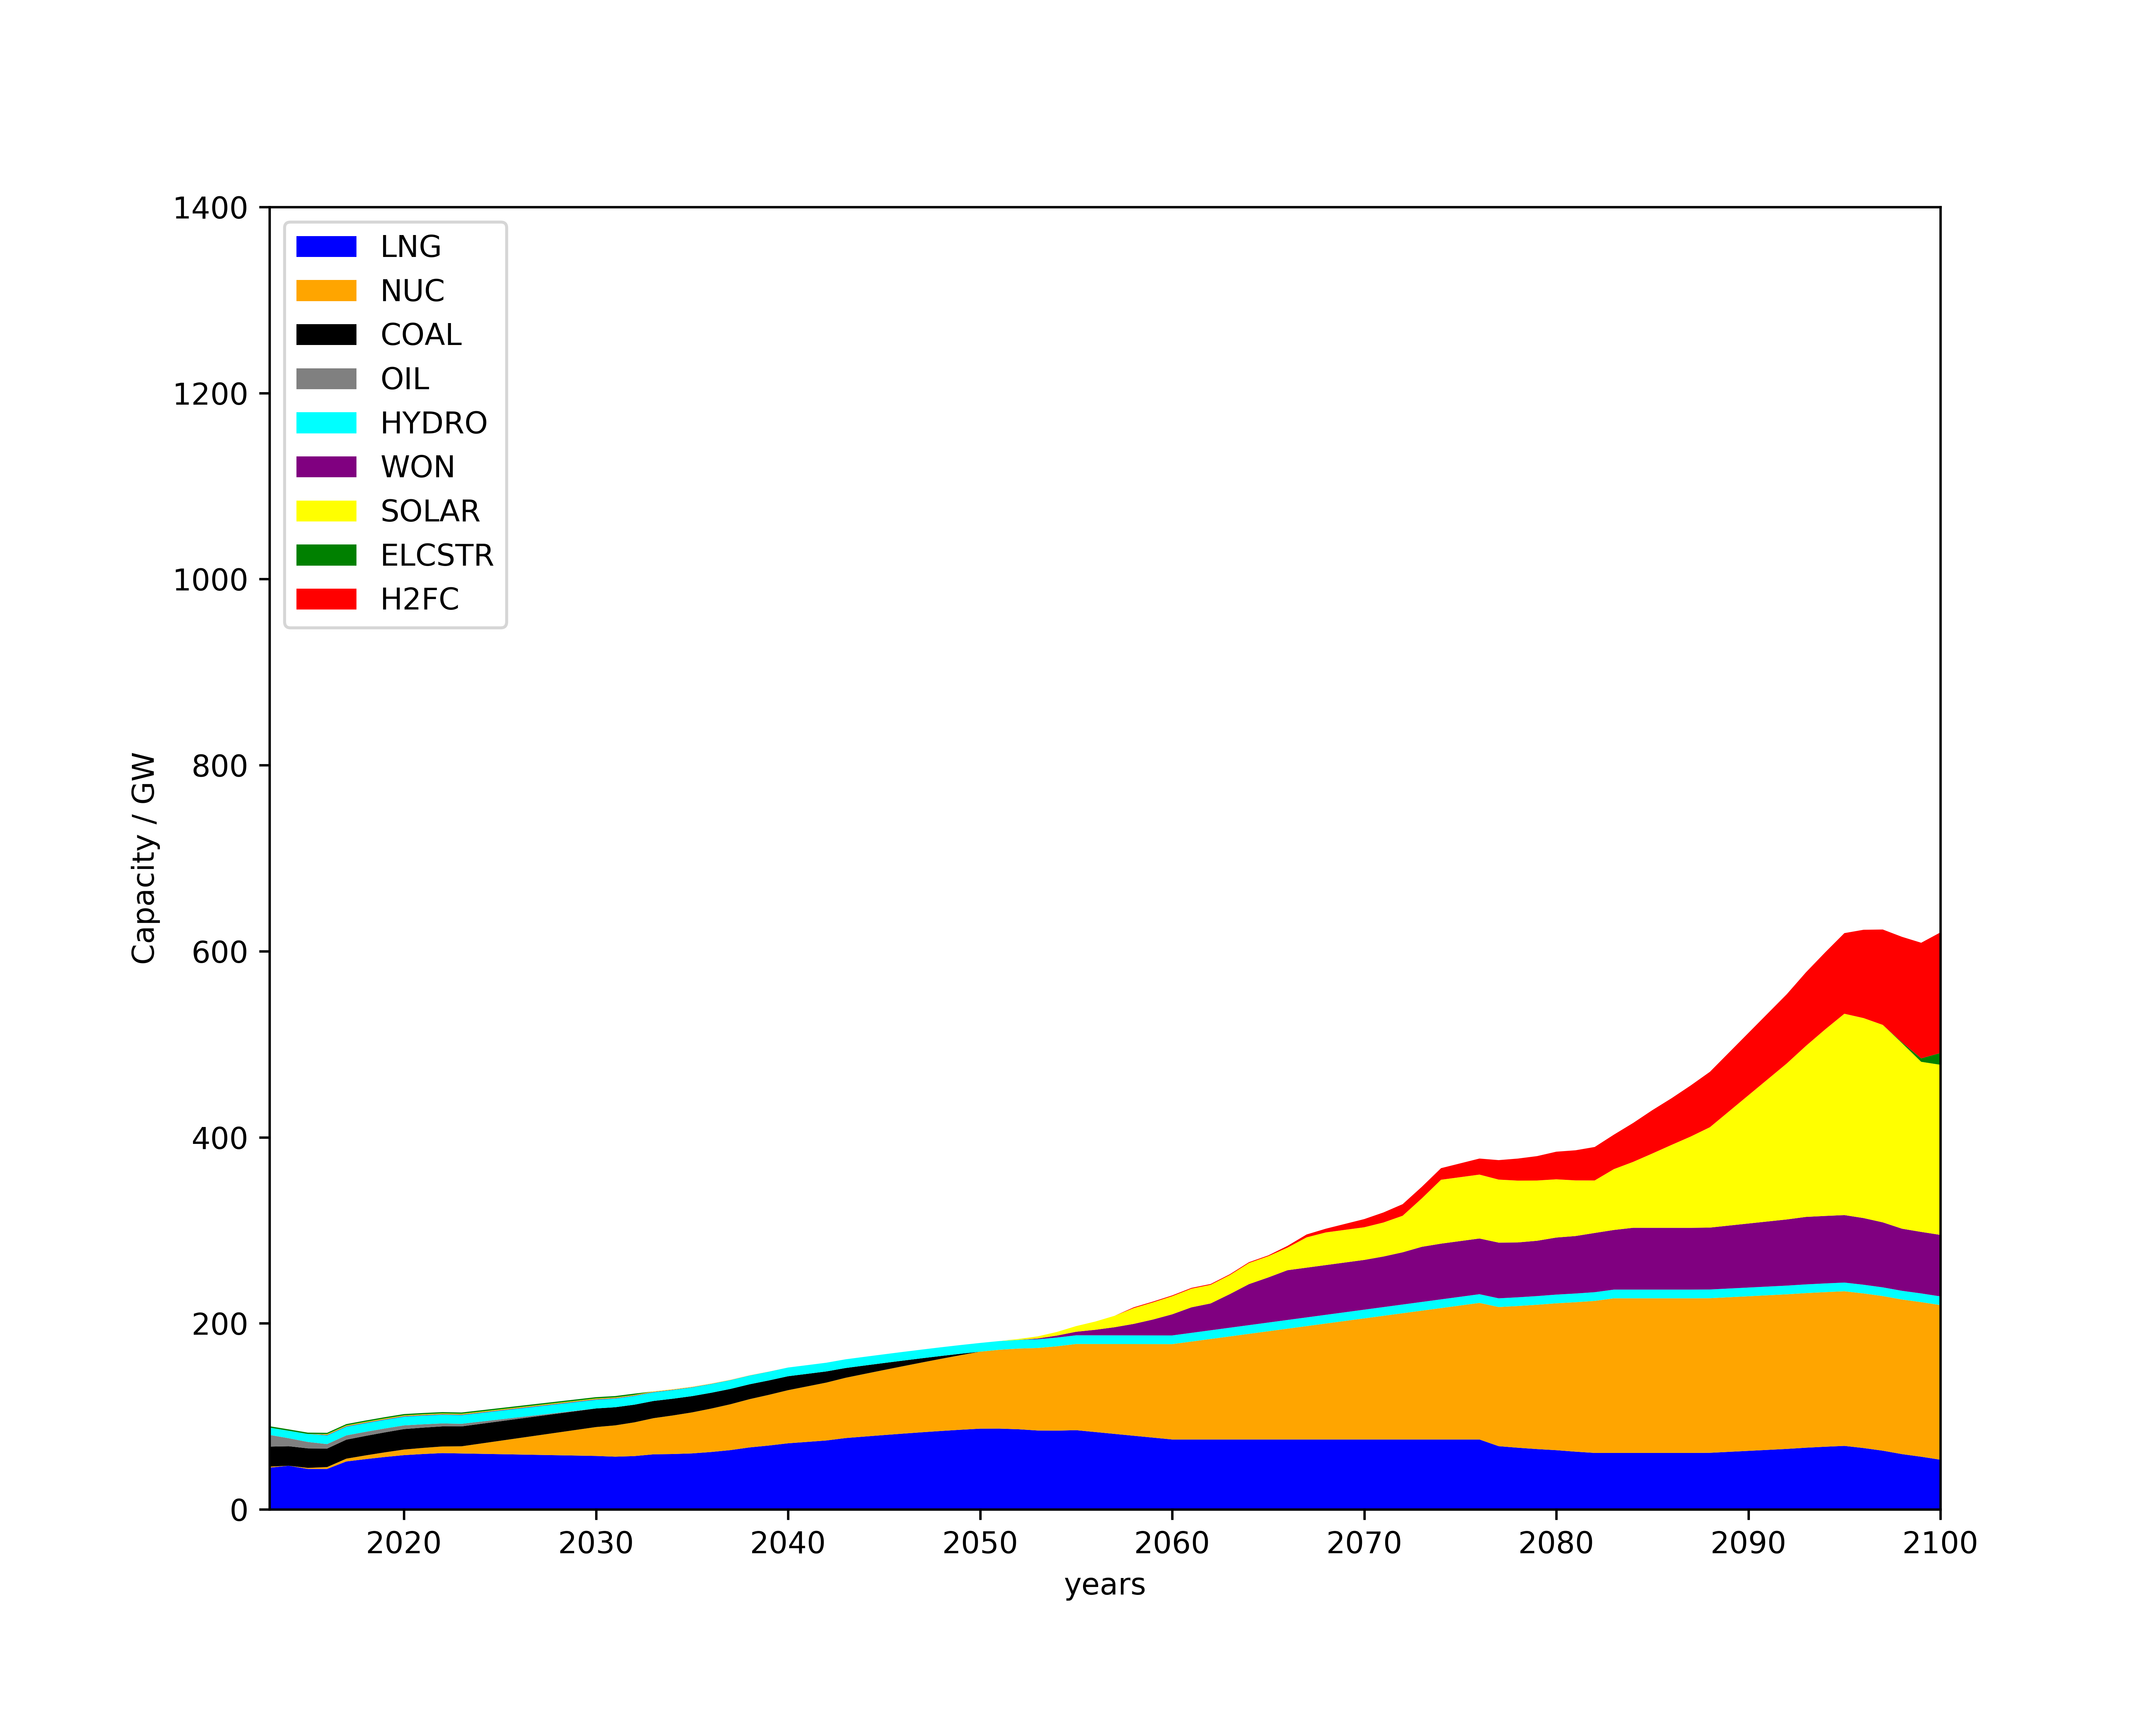
\includegraphics[width=0.9\textwidth]{./plot/nuc_cap.png}
  \caption{Installed capacity with new reactors.}
  \label{fig:nuccap}
\end{figure}

The actual electricity generated from different sources in the corresponding cases are shown in Figure.\ref{fig:nonucpower} and Figure.\ref{fig:nucpower}. It's clear that without nuclear energy, hydrogen fuel cell will replace natural gas not only as the back-up for solar and wind power, but also as the main electricity generating technology. Even in the case with new nuclear reactors, hydrogen fuel cells will generate comparable amount of electricity, suggesting the overall efficiency of hydrogen economy rivals nuclear energy, if high efficiency hydrogen production method is available.
\begin{figure}[H]
  \centering
    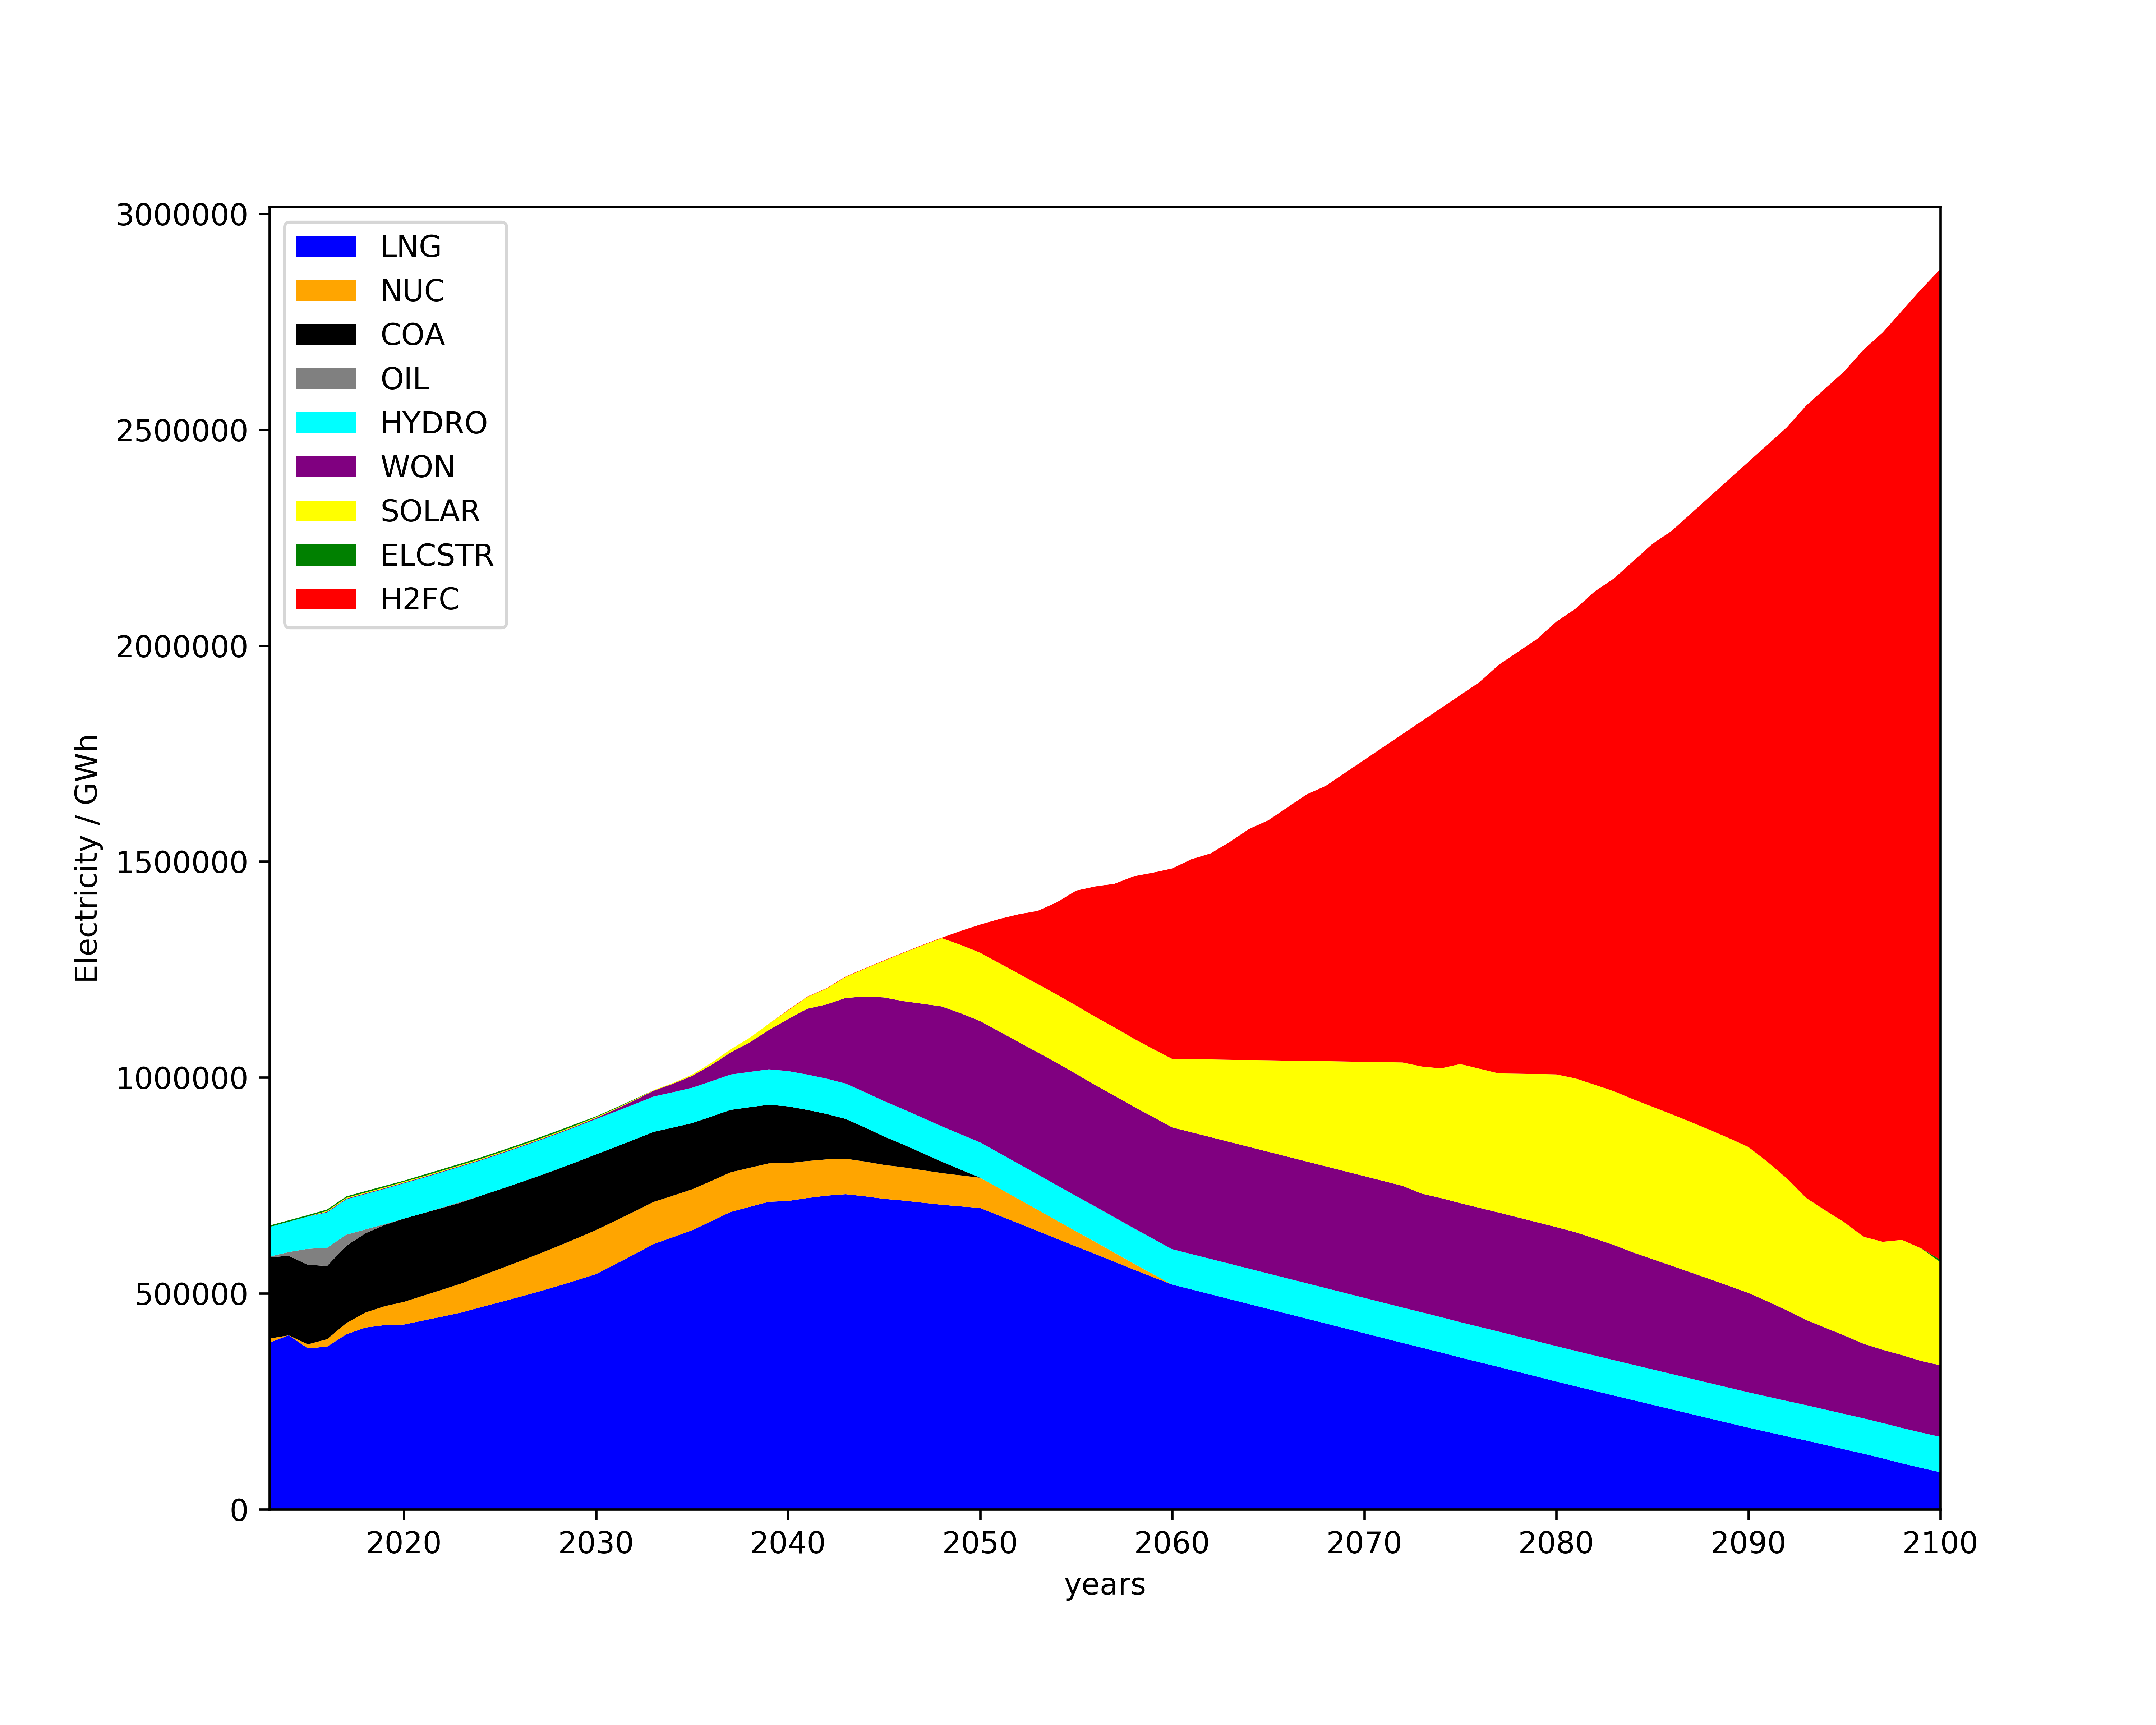
\includegraphics[width=0.9\textwidth]{./plot/nonuc_power.png}
  \caption{Electricity generated without new reactors.}
  \label{fig:nonucpower}
\end{figure}
\begin{figure}[H]
  \centering
    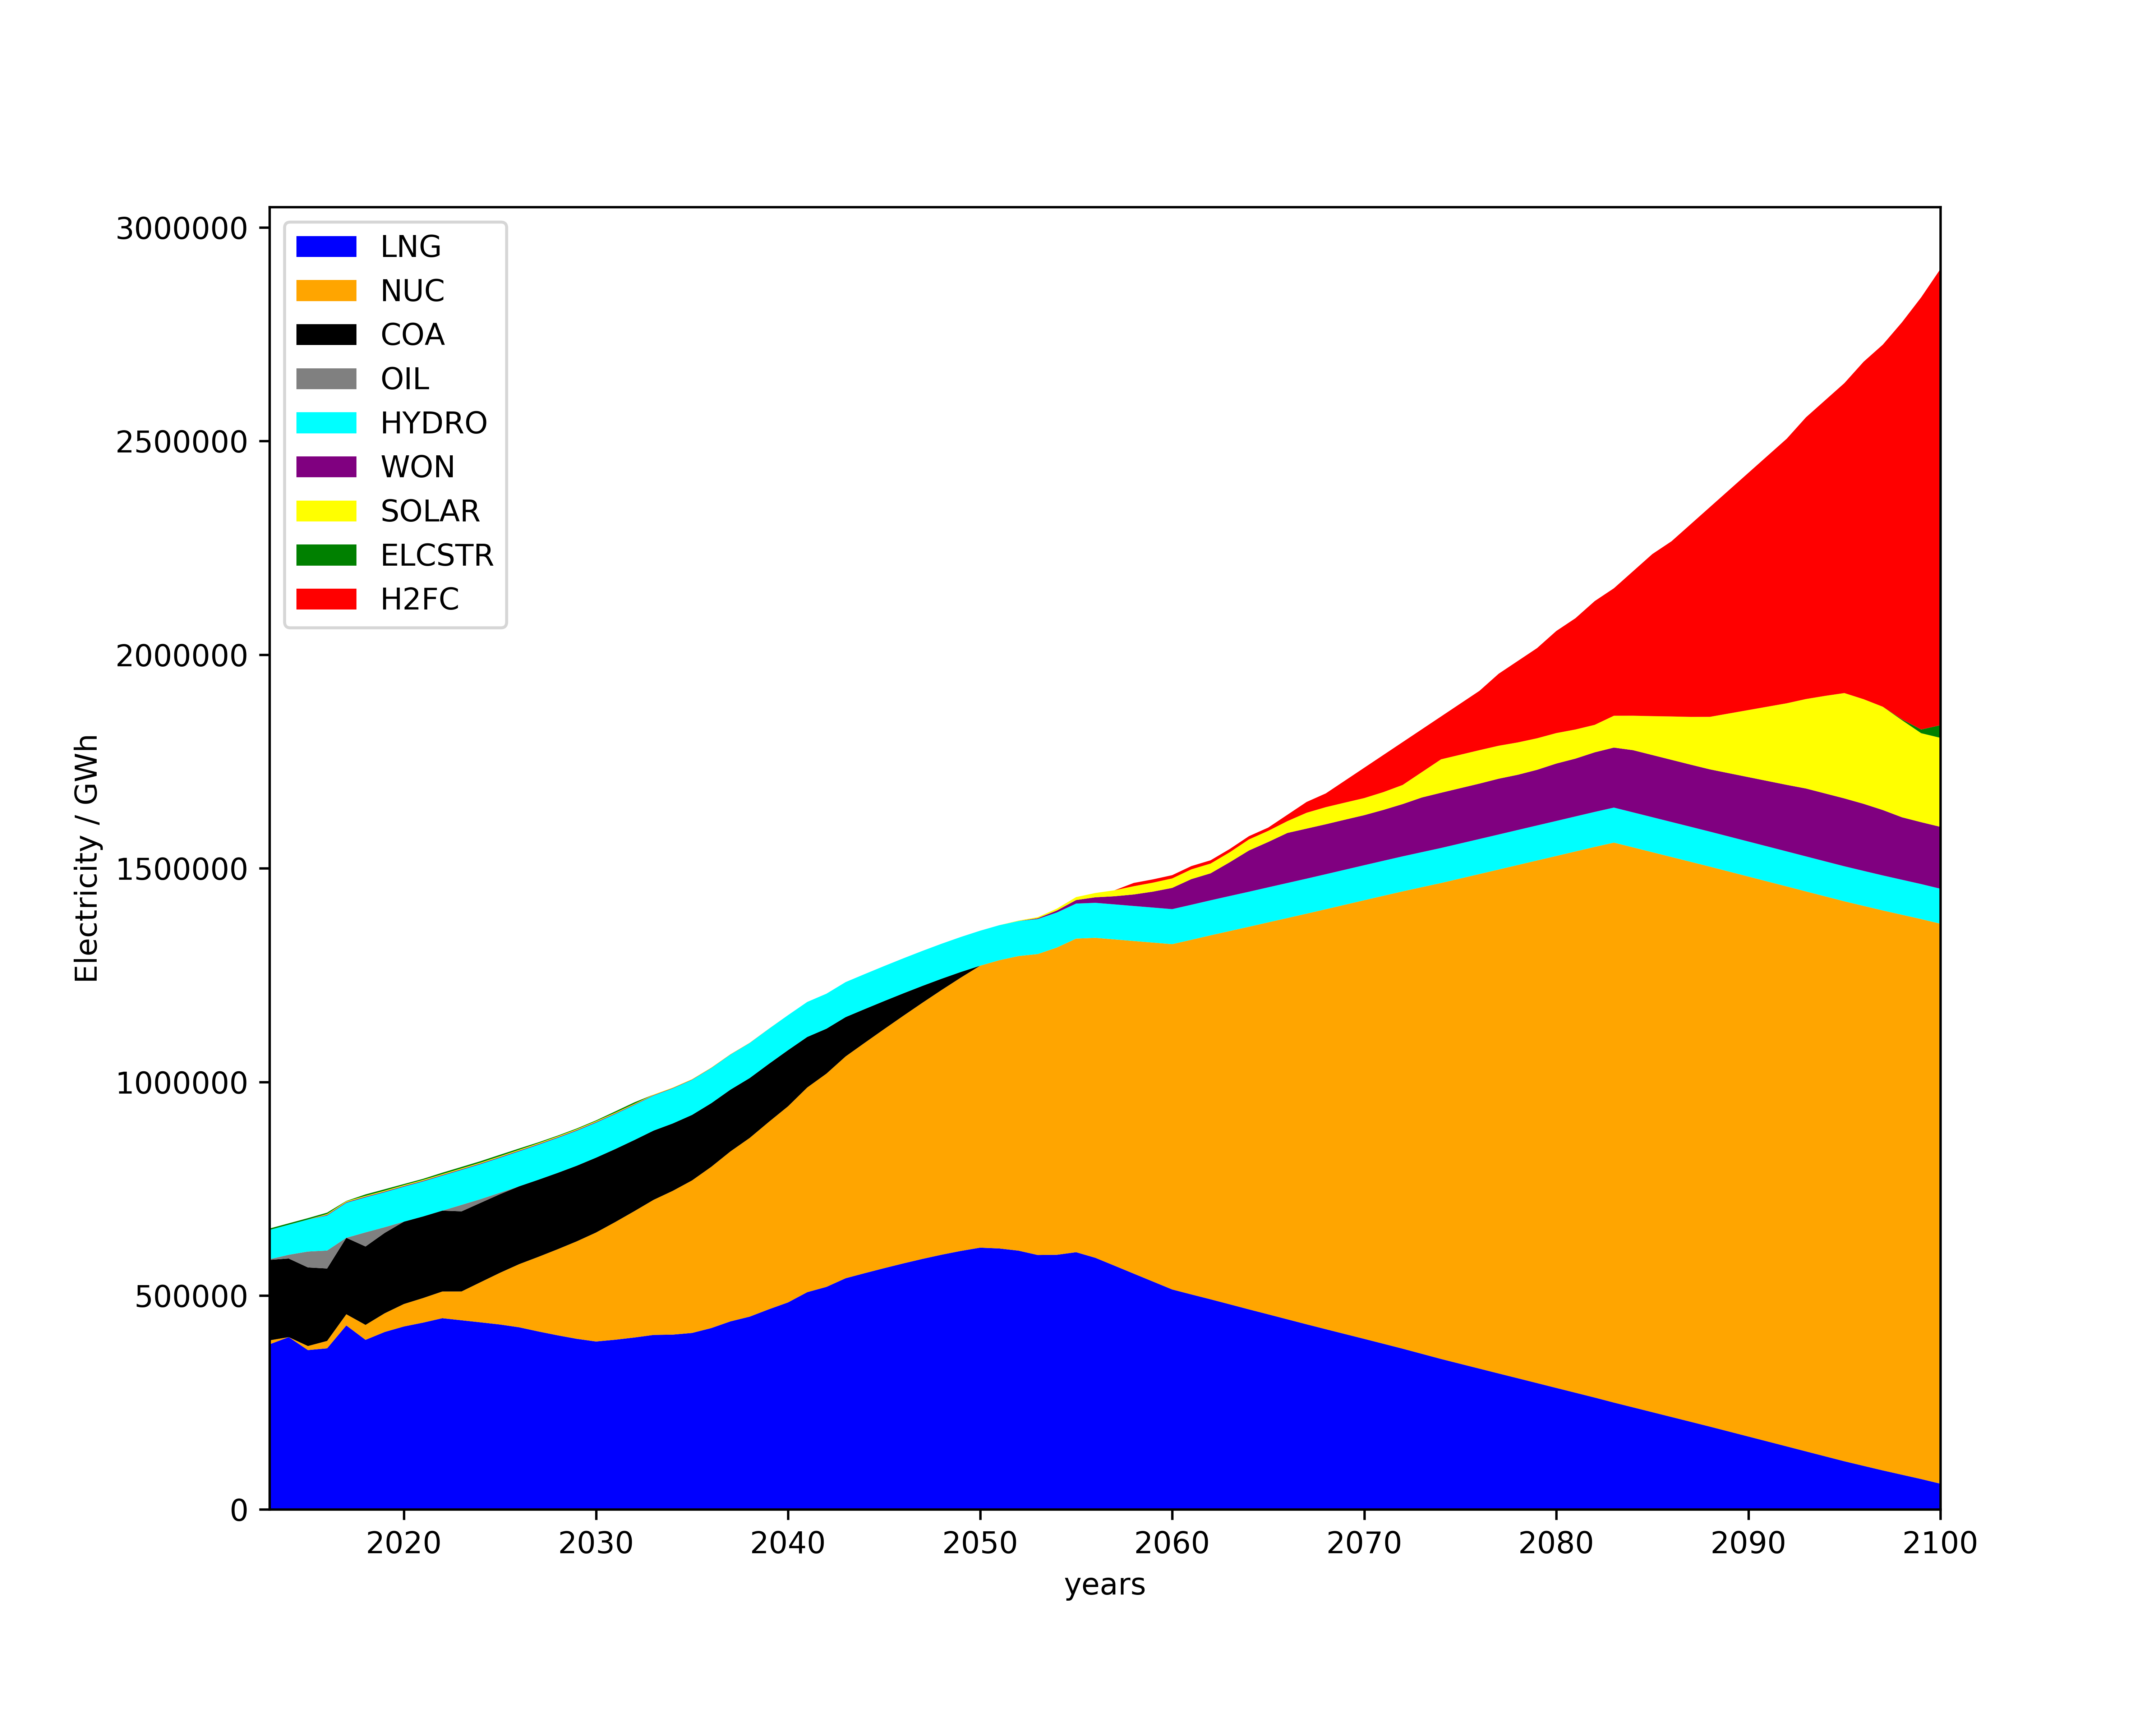
\includegraphics[width=0.9\textwidth]{./plot/nuc_power.png}
  \caption{Electricity generated with new reactors.}
  \label{fig:nucpower}
\end{figure}

\subsection{Carbon Emission}
The carbon emission from electricity generation sector is shown in Figure.\ref{fig:nonucco2} and Figure.\ref{fig:nucco2}. These two figures illustrate the significance of the definition of carbon reduction pathway. Because of the intermittent characteristics of wind and solar power, part of the energy demand must be met by burning fossil fuel. Under the assumption of increasing power demand by 1.7\% each year and maximum growth rate of new capacity by 30\% each year, it's inevitable that the carbon emission will continue to increase until renewable energy reach some critical level. In the case without new nuclear reactor, the carbon emission will continue to increase at a faster pace until it reach the maximum emission around 2040. By then the emission will be increased by 100\% compared the base year level. In both cases the emission by 2050 will be inceased by 50\%. Comparing two emission profiles side by side, it's clear that the higher emission in the no nuclear case is mainly due to burning coal. Note that there's no new coal capacity. All electricity generated from burning coal is from the exisiting capacity.


\begin{figure}[H]
  \centering
    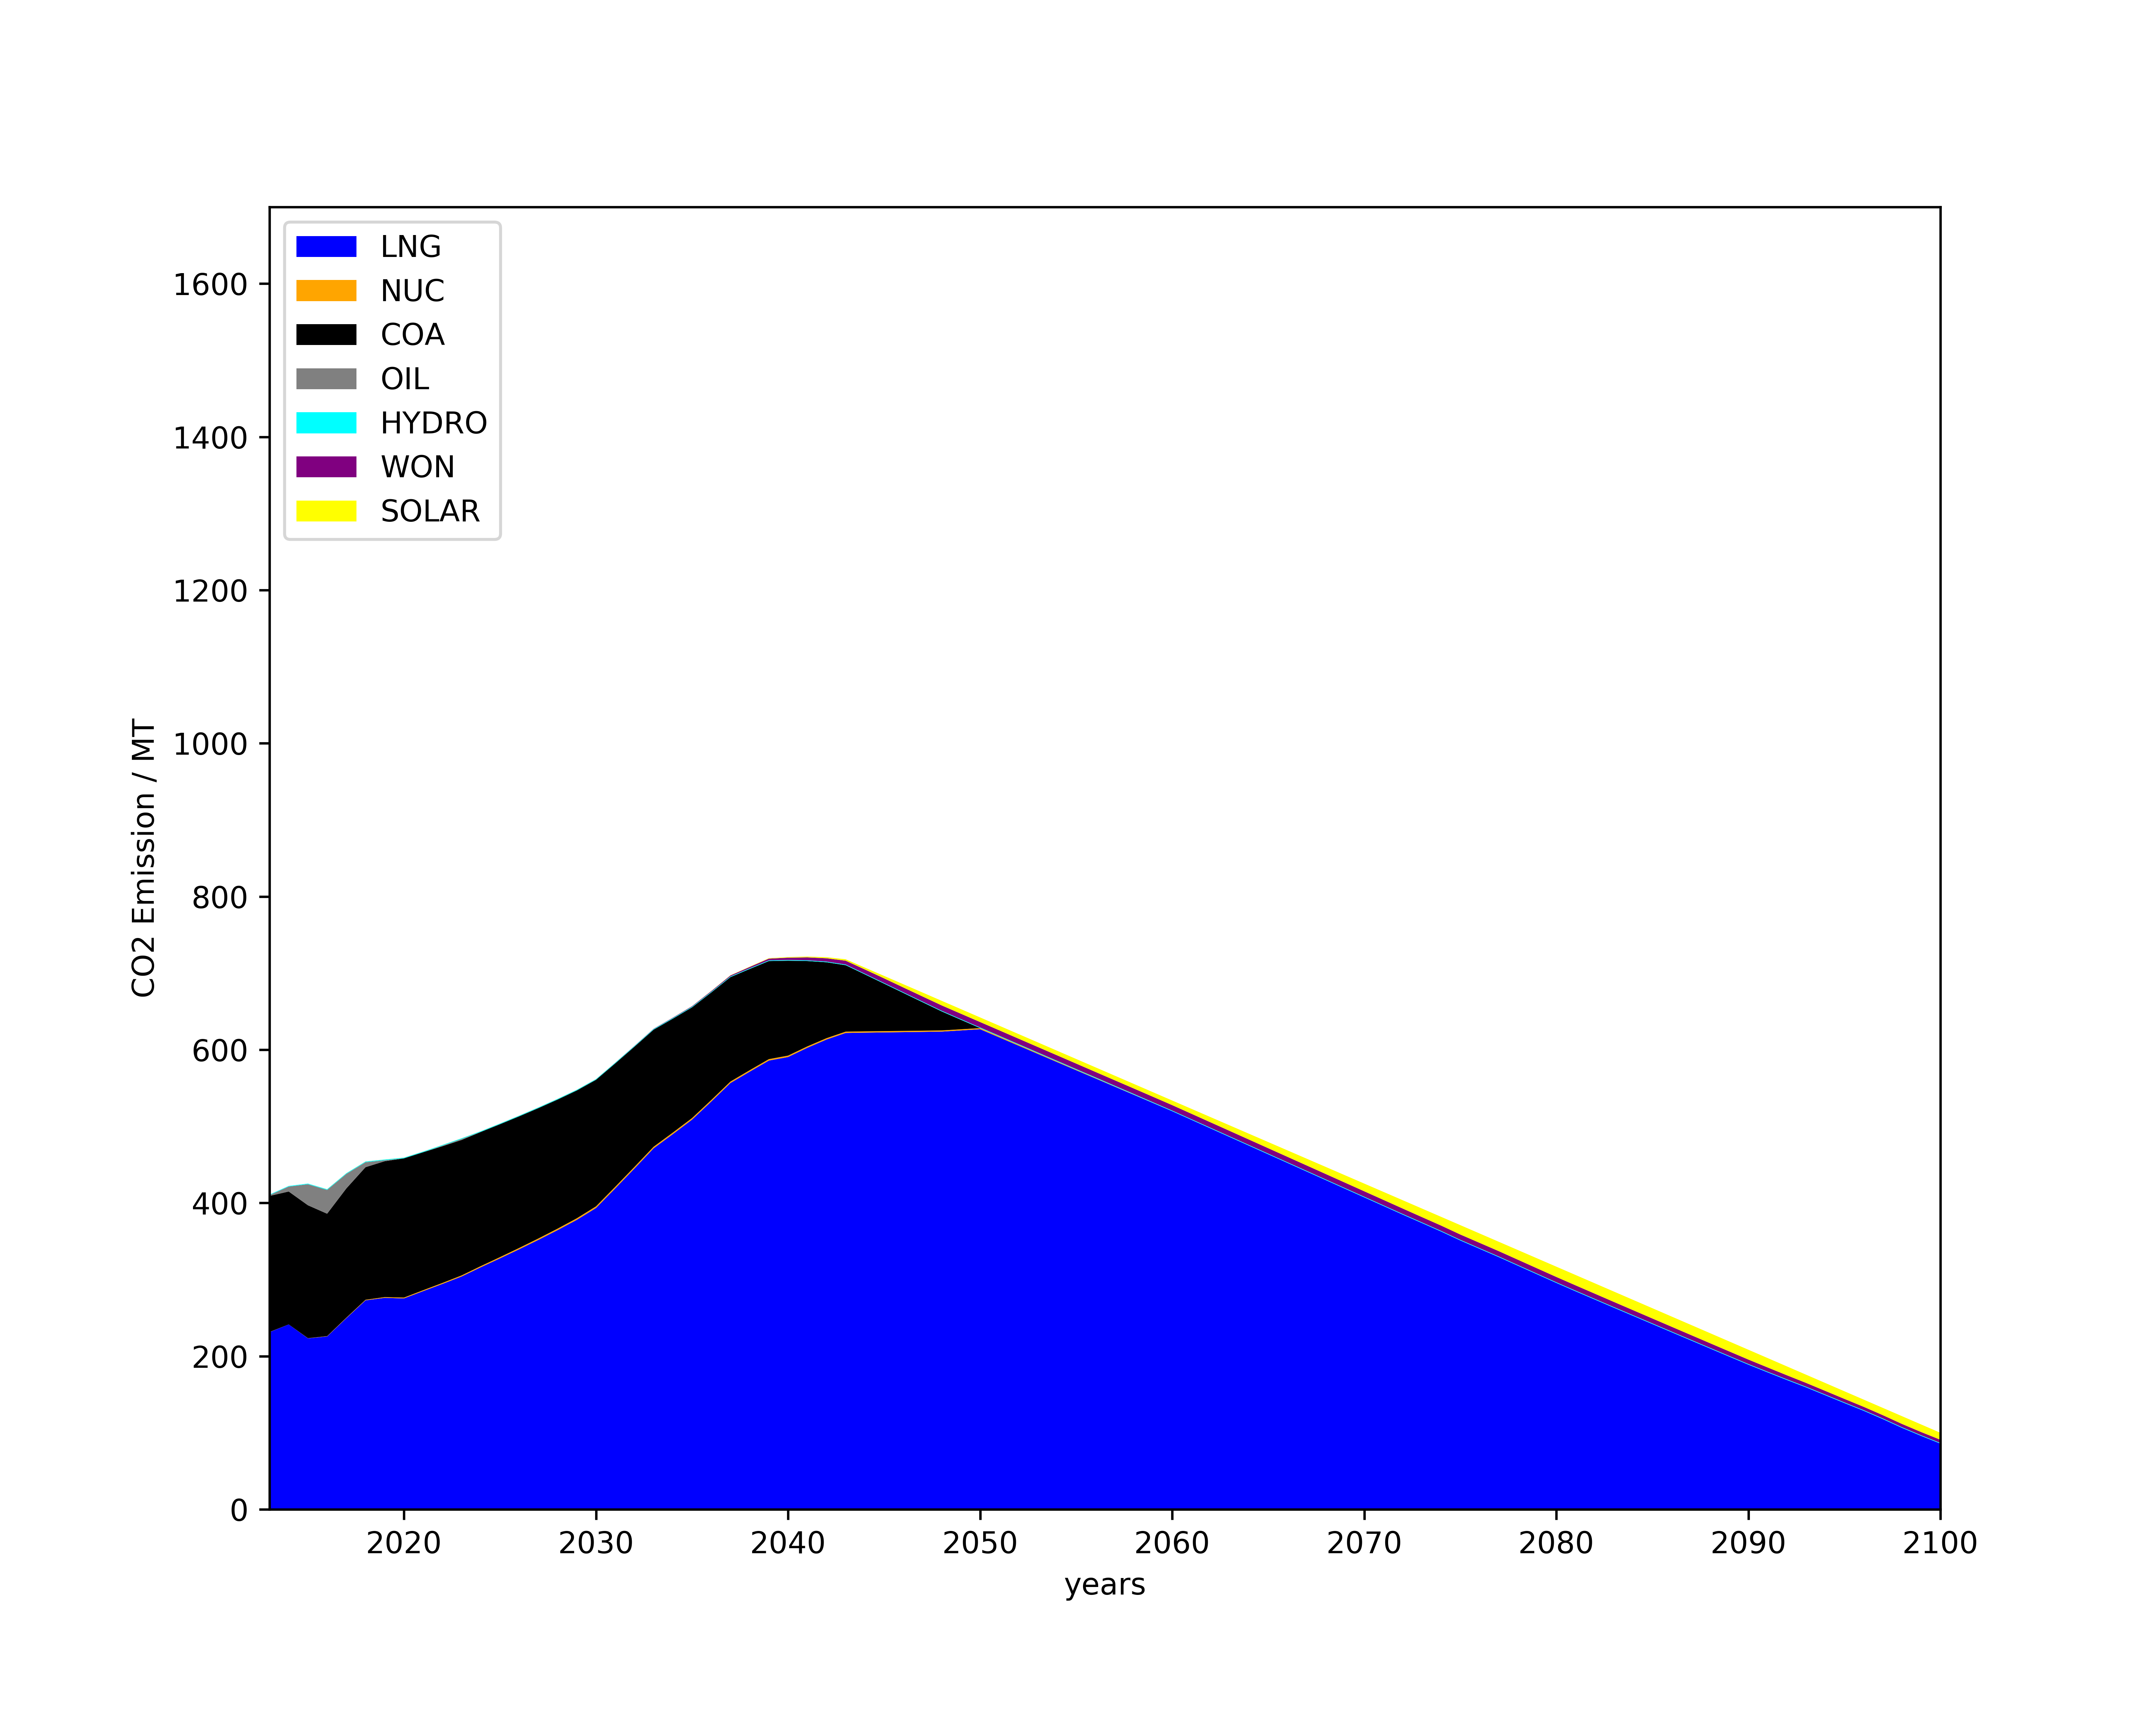
\includegraphics[width=0.9\textwidth]{./plot/nonuc_co2.png}
  \caption{Carbon emission in electricity generation sector without new reactors.}
  \label{fig:nonucco2}
\end{figure}
\begin{figure}[H]
  \centering
    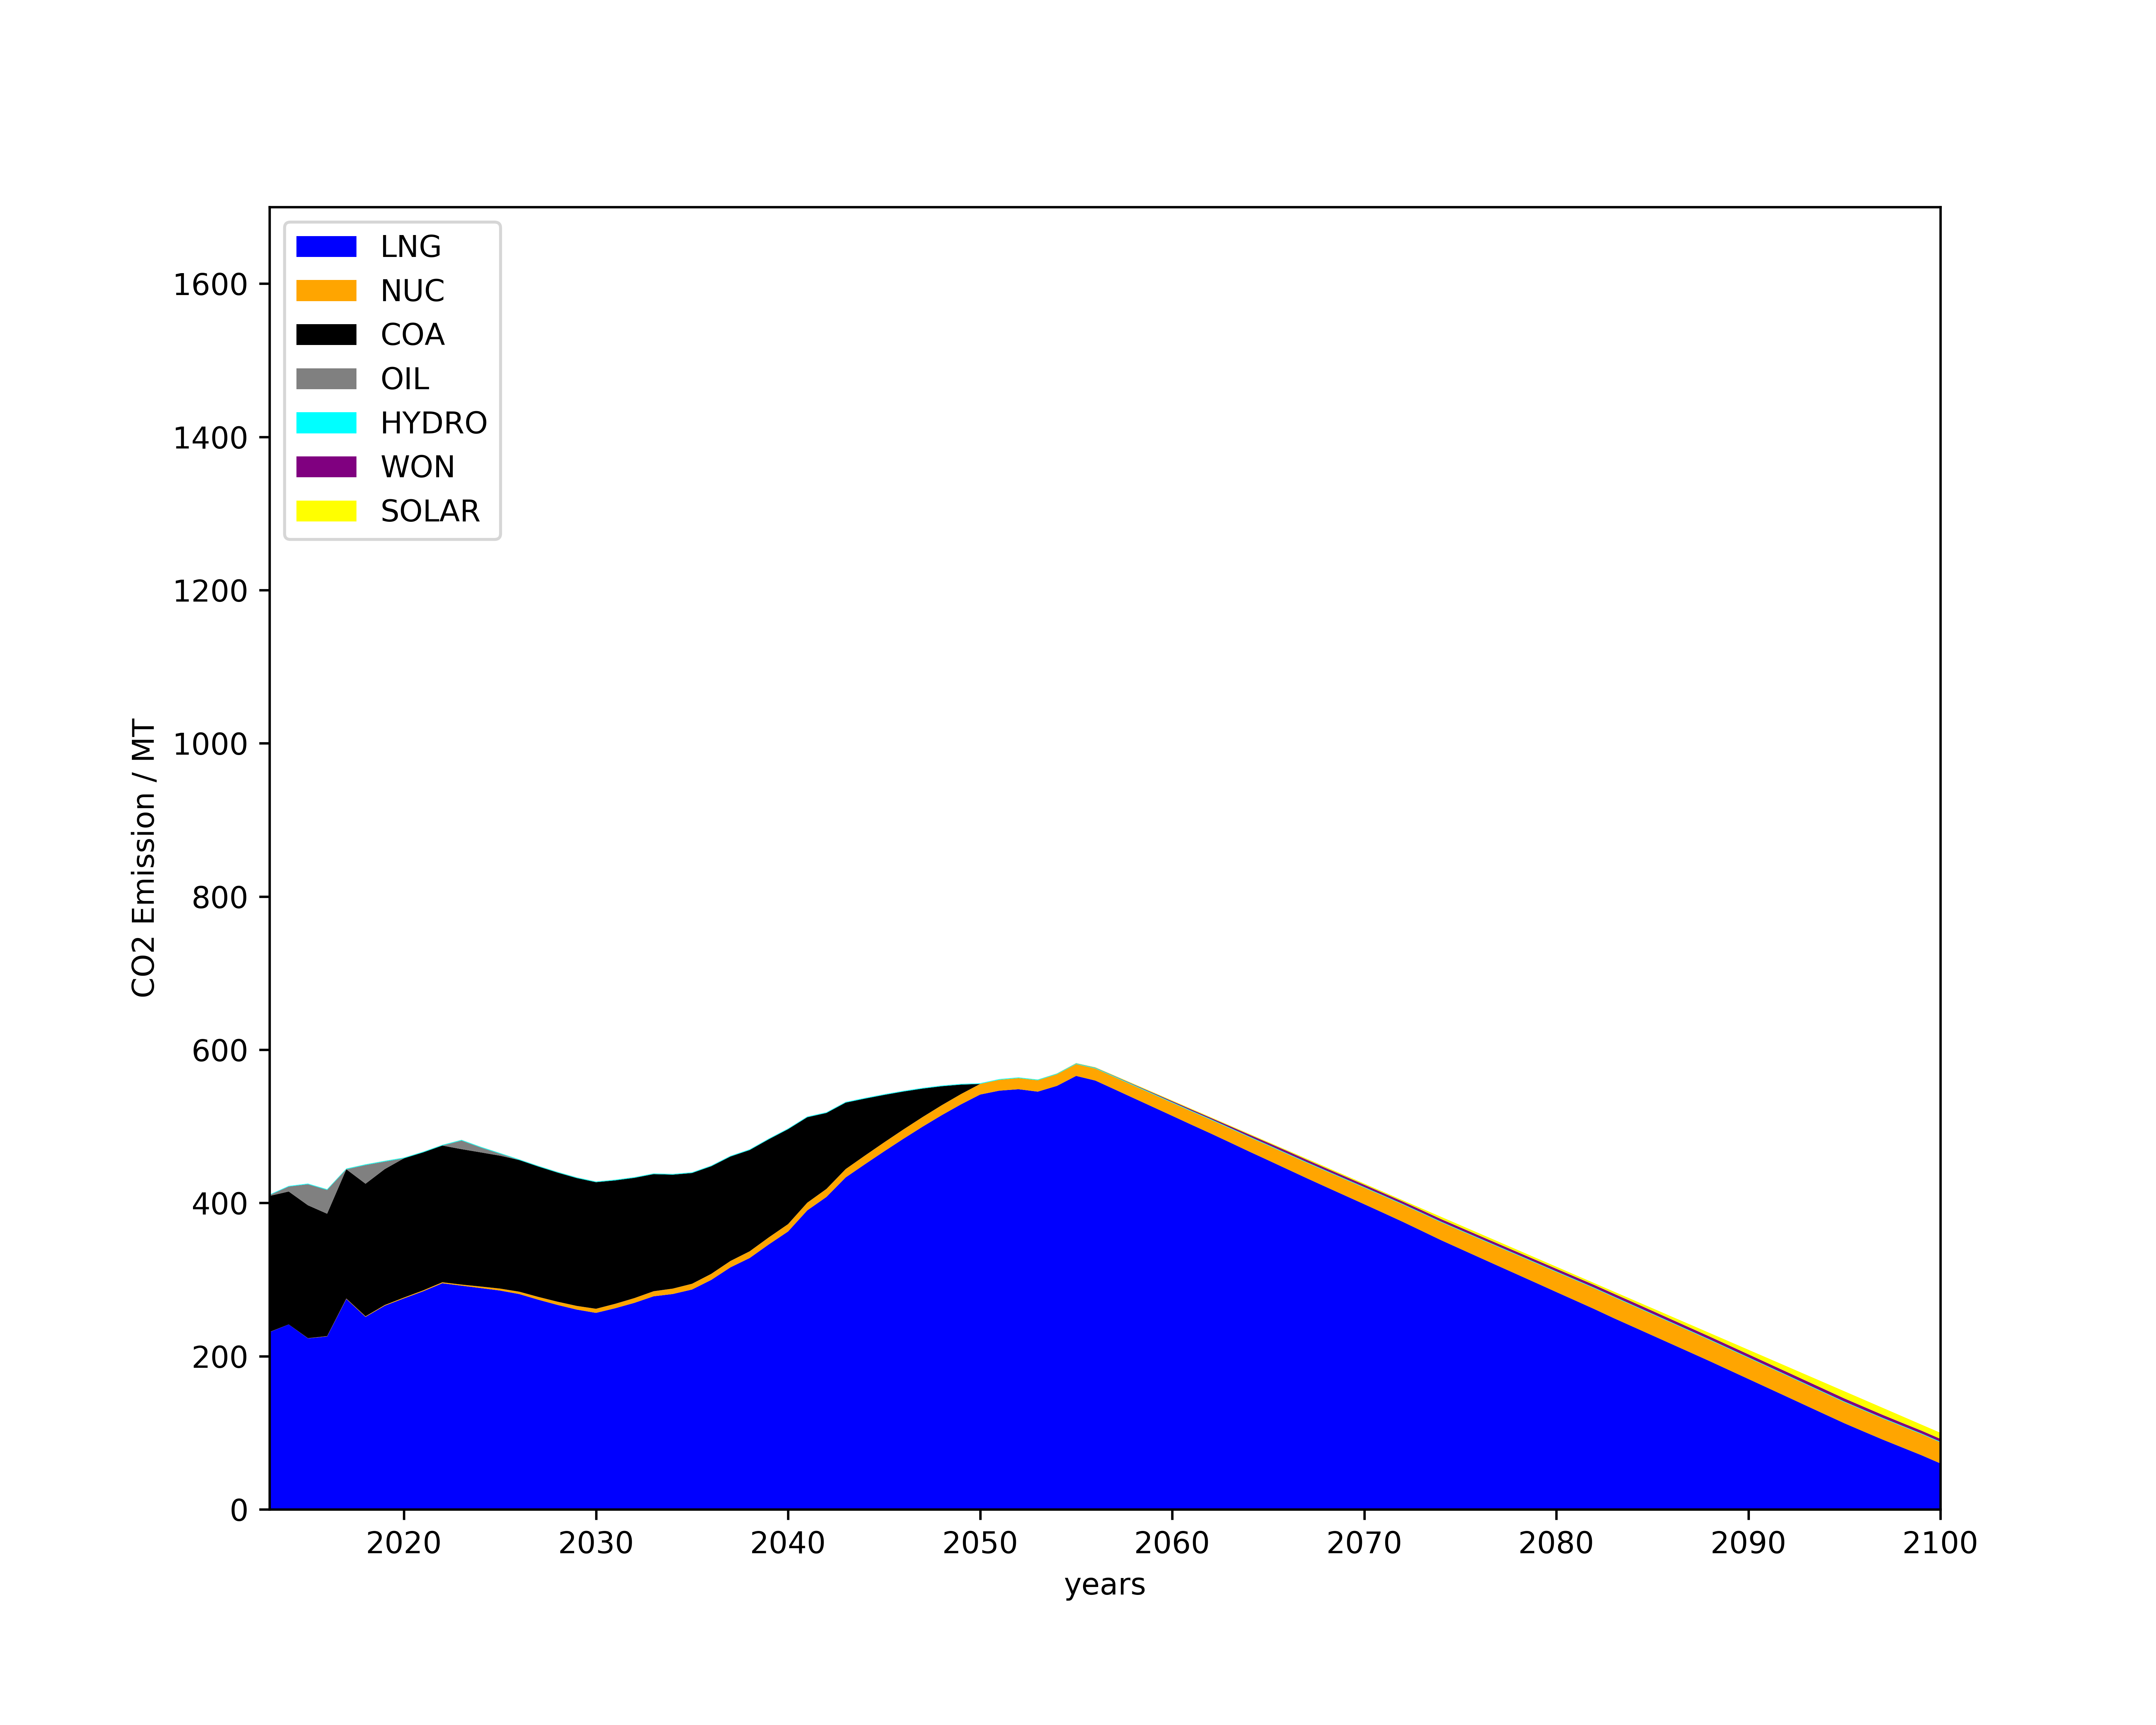
\includegraphics[width=0.9\textwidth]{./plot/nuc_co2.png}
  \caption{Carbon emission in electricity generation sector with new reactors.}
  \label{fig:nucco2}
\end{figure}


\subsection{Personal Vehicle Composition}

In the current model, the transportation sector is relatively simple compared to electricity sector. The demand is assumed to be constant and only three types of vehicles is modeled. It is assumed that the performance and cost of these vehicles will converge to the same level by 2030. It turns out that there's no impact from the absence of new nuclear reactor when it comes to composition of personal passenger vehicles. The change of number of passenger vehicle is identical in both cases and is shown in Figure.\ref{fig:nonuccar}.
There are two clear transitions in vehicle composition. The conventional gasoline vehicle will firstly be replaced by electric vehicle. All gasoline vehicles will be completely replaced by electric car and hydrogen fuel cell car by mid 40s. After that electric cars start to retire and will be all replaced by hydrogen fuel cell vehicle after 2060.


\begin{figure}[H]
  \centering
    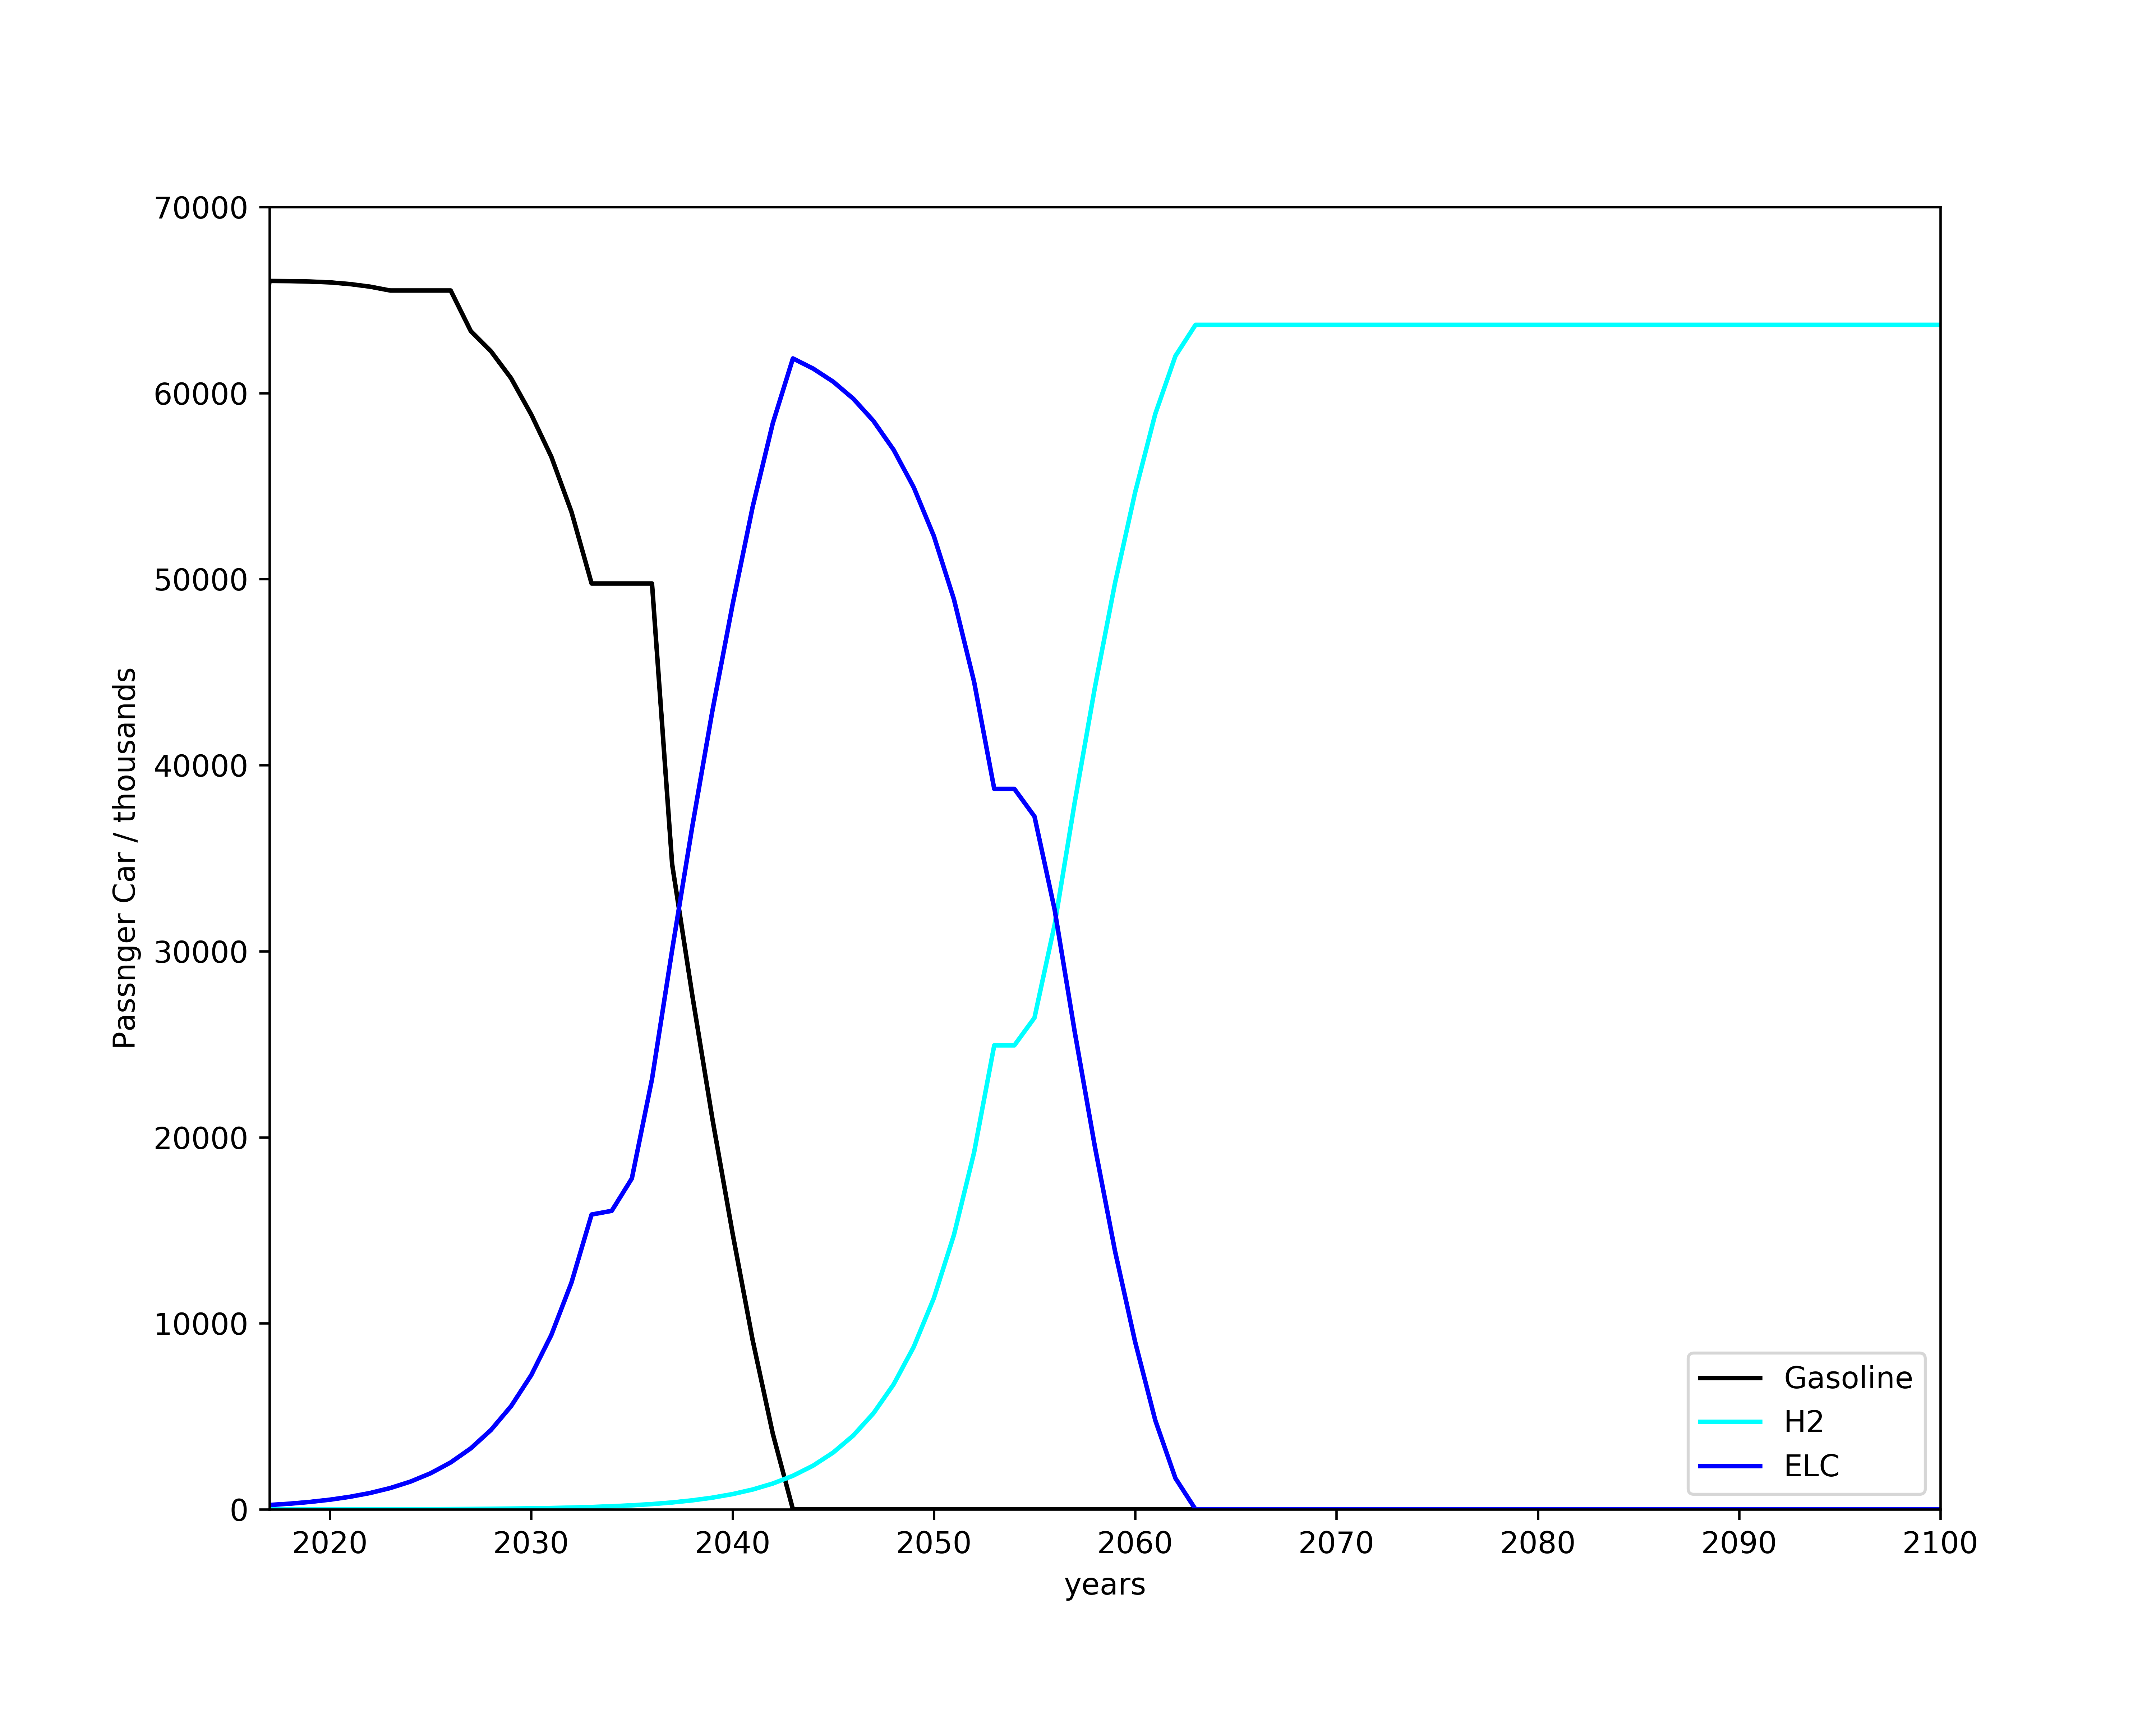
\includegraphics[width=0.9\textwidth]{./plot/nonuc_car.png}
  \caption{Total number of personal vehicles.}
  \label{fig:nonuccar}
\end{figure}


\subsection{Hydrogen Production and Storage}
\label{sec:hydrogen production}

Finally the means of hydrogen production will be presented. As shown in Figure.\ref{fig:nonuch2} and Figure.\ref{fig:nuch2}, in both scenarios hydrogen production only increase after photocatalysis is available. The cost of photocatalysis is estimated to be 2.0\$ per kilogram of hydrogen\cite{pinaud2013technical}. Clearly before the introduction of advanced production method, there's no economical advantage of switching to hydrogen economy. The overall system efficiency of converting natural gas to hydrogen is lower than converting it to electricity. The PV-electrolysis system is also of low efficiency so the electrolysis process is not activated by the model. Since photocatalysis is modeled in a similar way as solar power, it requires hydrogen storage device to store the hydrogen produced in the morning. In both cases, all hydrogen usage is either coming from production of photocatalysis or hydrogen storage. Under no nuclear assumption the demand for hydrogen is significantly larger.
\begin{figure}[H]
  \centering
    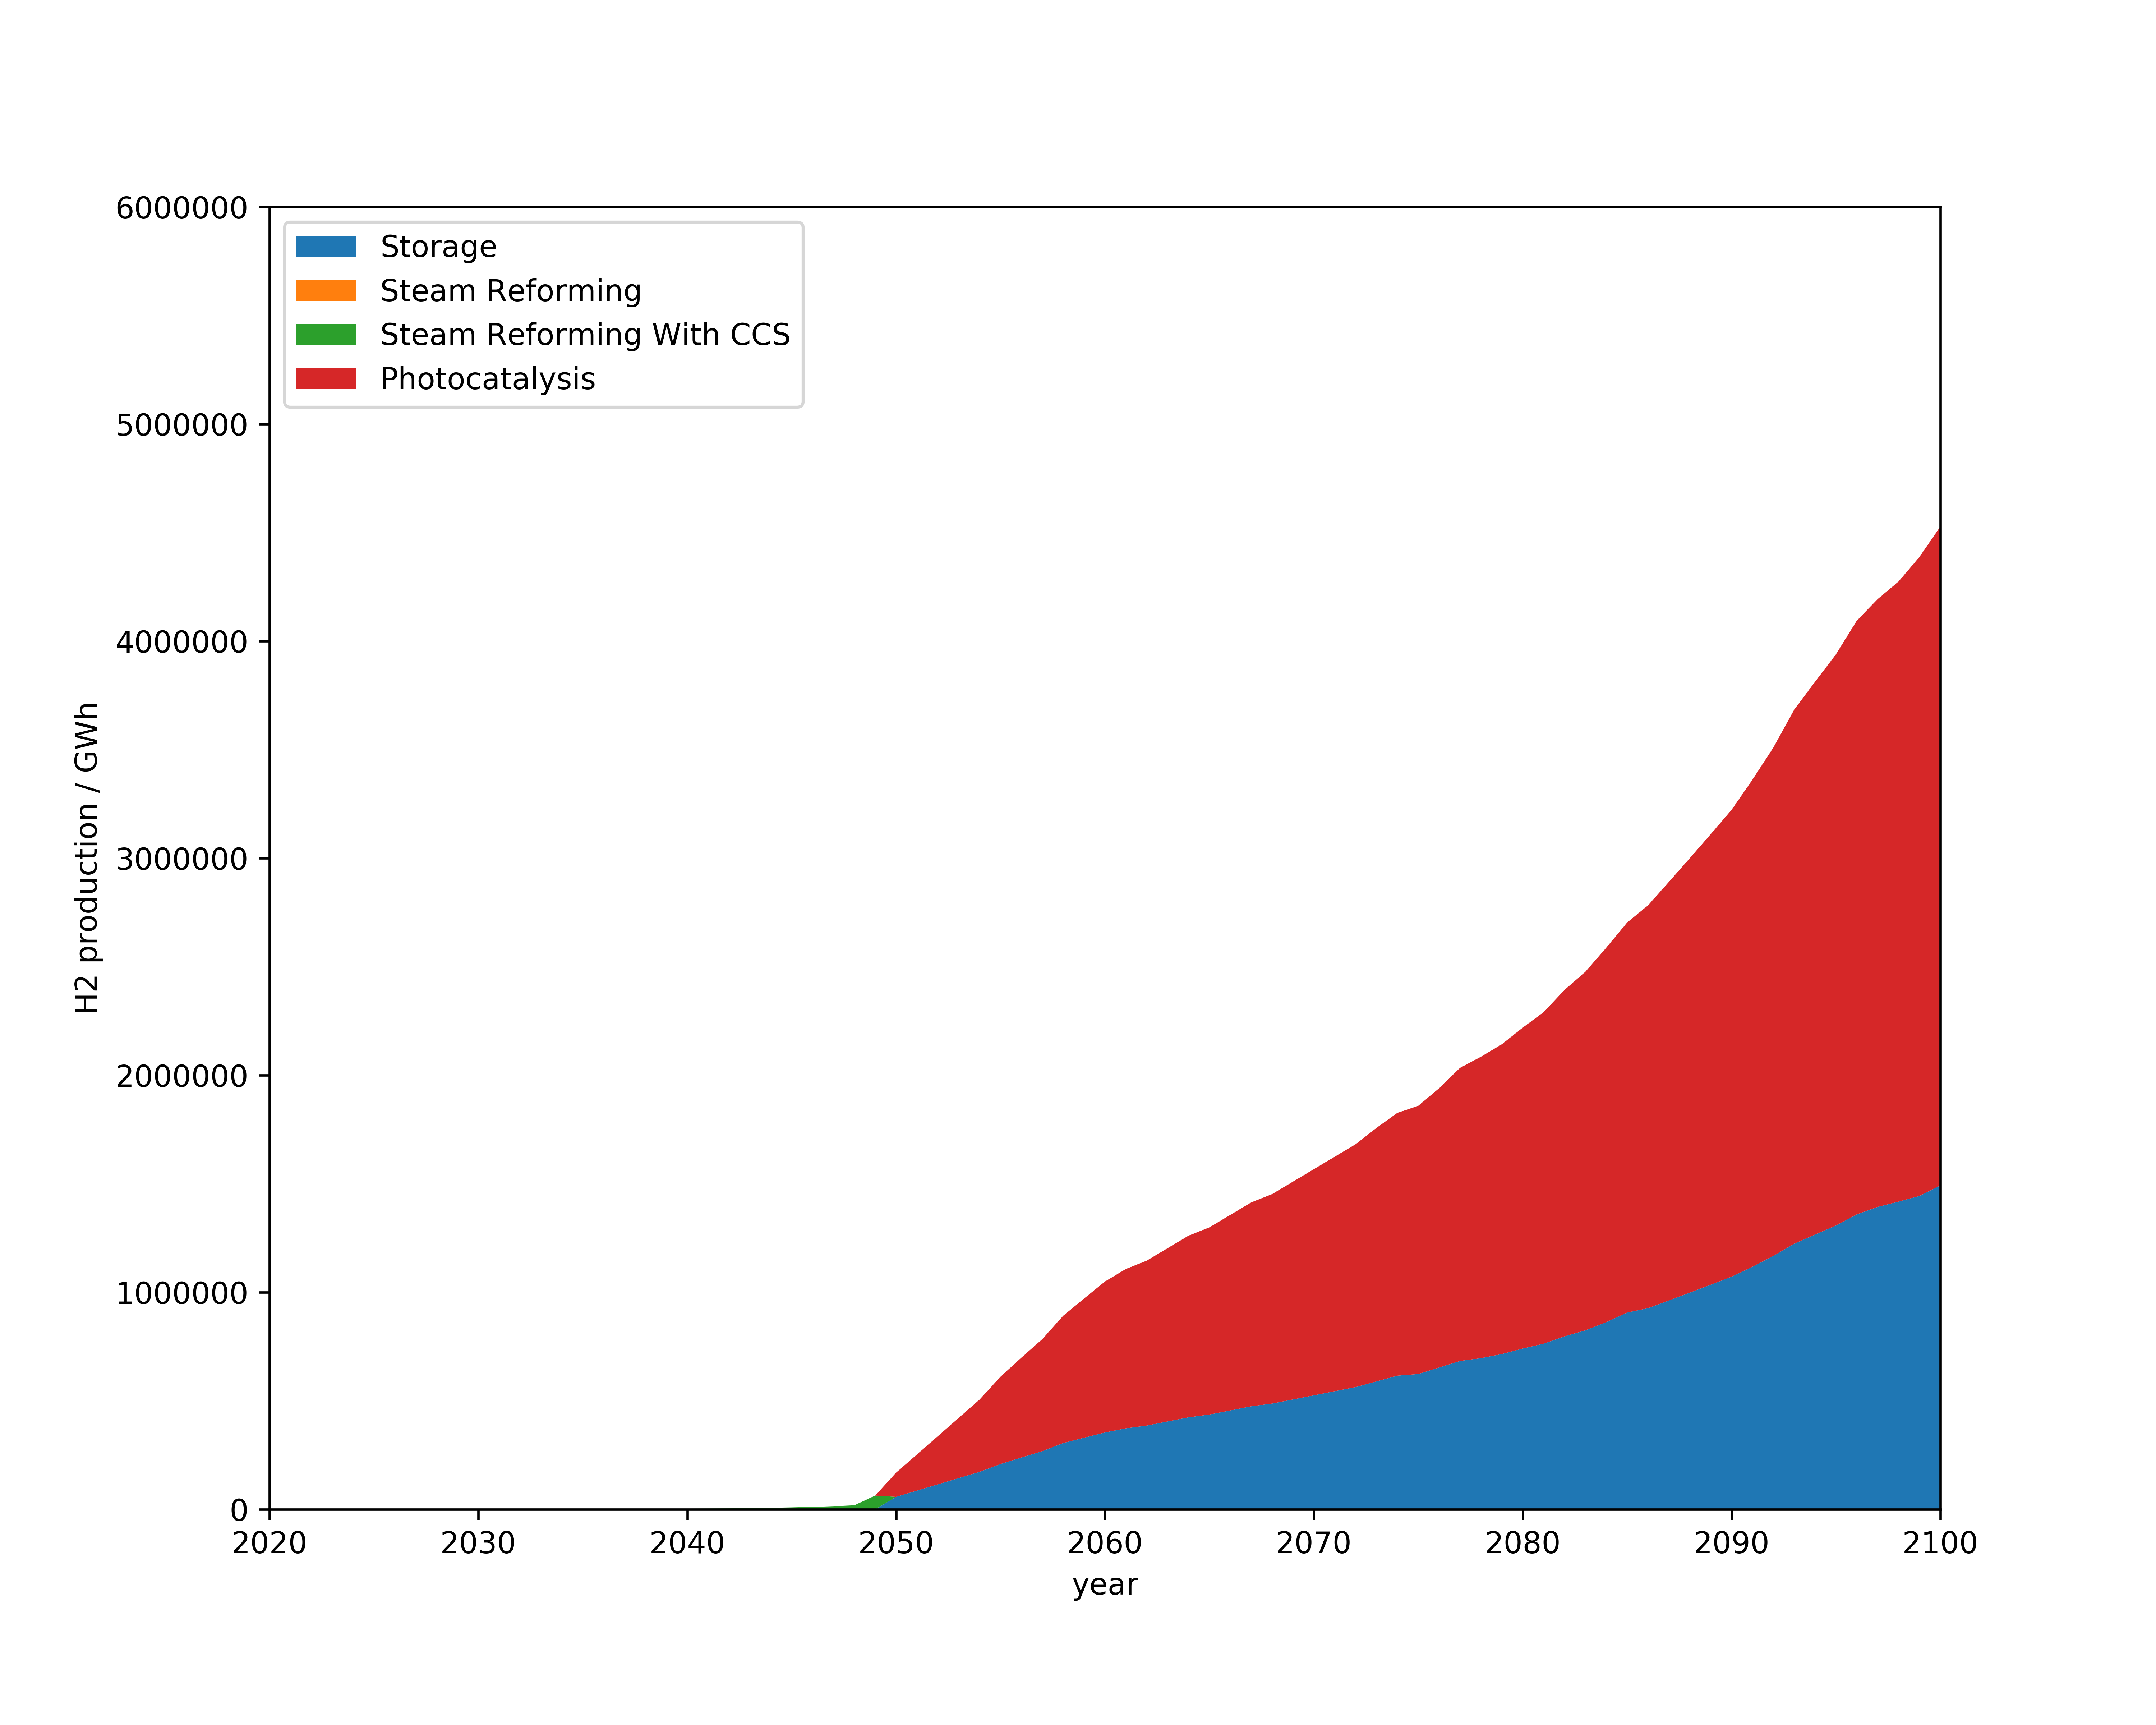
\includegraphics[width=0.9\textwidth]{./plot/nonuc_h2.png}
  \caption{Total hydrogen output by source without new reactors}
  \label{fig:nonuch2}
\end{figure}
\begin{figure}[H]
  \centering
    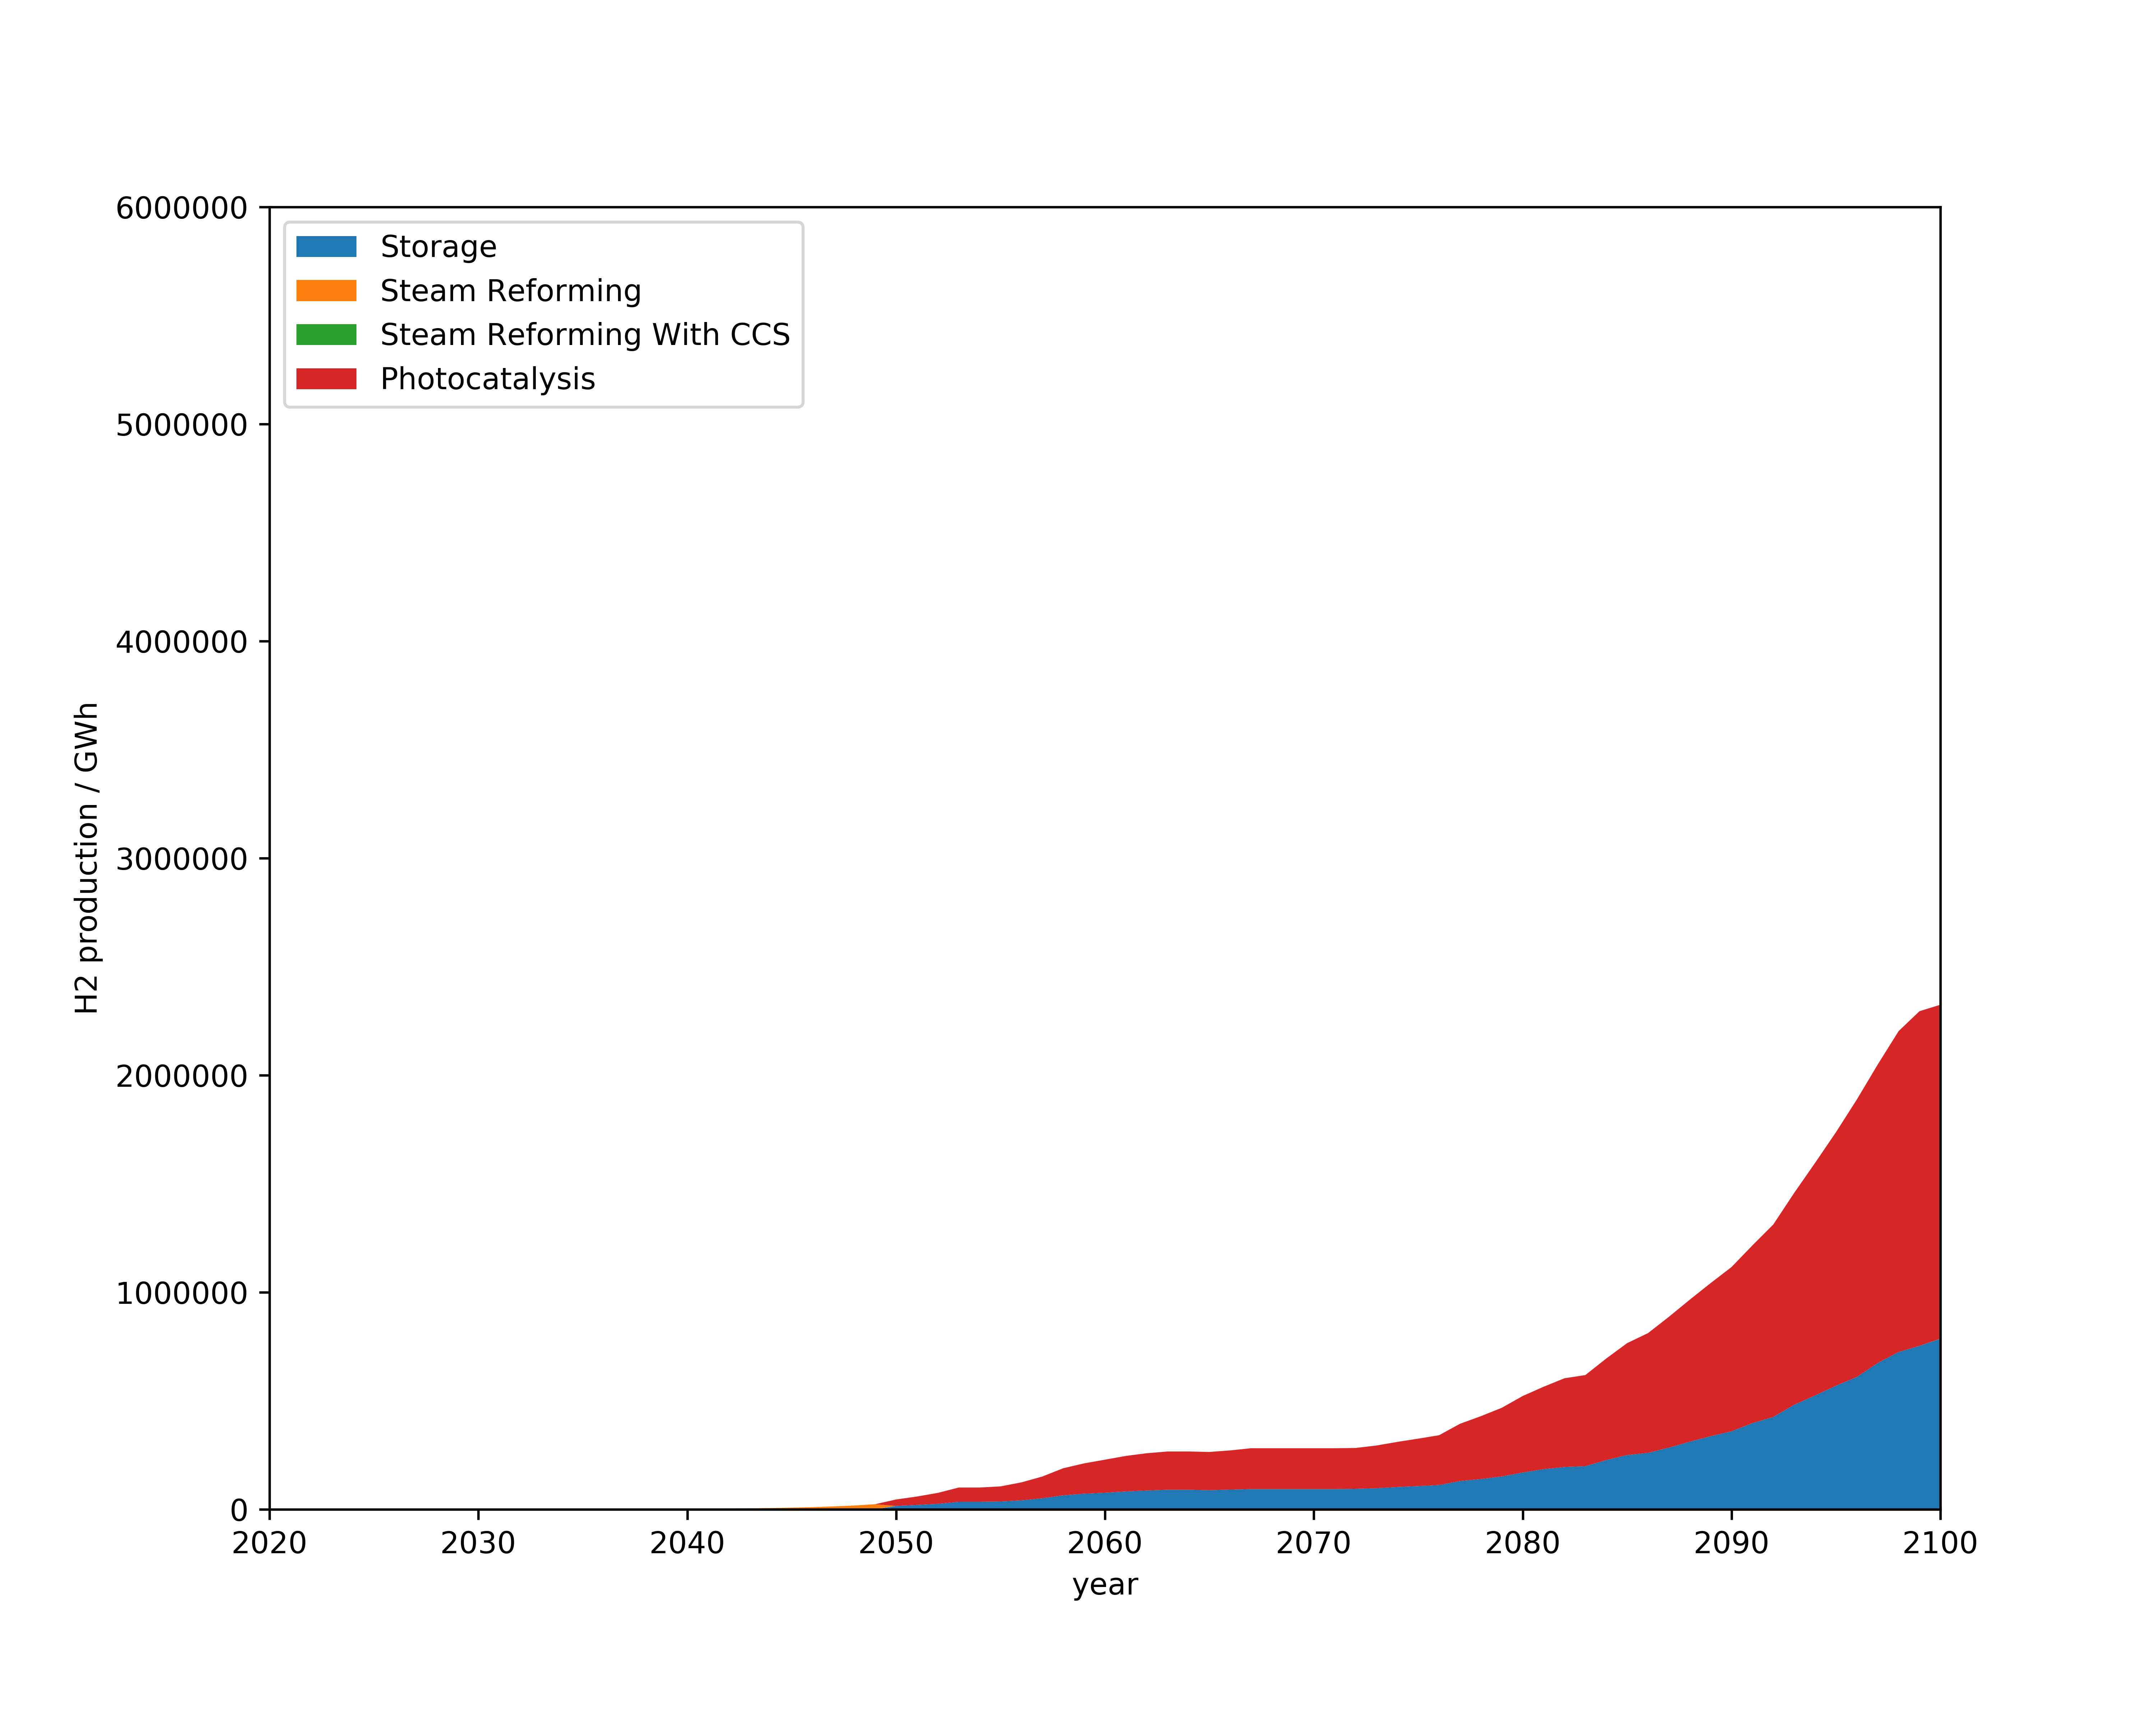
\includegraphics[width=0.9\textwidth]{./plot/nuc_h2.png}
  \caption{Total hydrogen output by source with new reactors}
  \label{fig:nuch2}
\end{figure}



\section{Future Work}
The current model have included sufficient TIMES functions to model the energy structure transitions. The future work should focus on data validating and adding detailed processes.

\subsection{Fuel Supply Curve}
Compared to the previous model, the fuel cost is now considered separately. The fuel cost is a crucial part in determining the overall cost of system, along with other factors such as efficiency and pathway. In Japan's case all fuels are imported. Detailed price information including exporting countries and corresponding prices can be included based on Japan's fuel import history.

\subsection{Transportation Sector}
The current transportation sector model only considers personal vehicle and three types of vehicle. More details can be added to the transportation part:
\subsubsection{Personal Passenger Transportation}
More vehicle types can be added to the personal passenger sector. In Japan's case it would be appropriate to add hybrid vehicles and plug-in hybrid electric vehicles. The detailed parameters need to be updated according to the estimations from Japan's strategic plan. 
\subsubsection{Public Passenger Transportation}
Modeling of public transportation sector includes railway and bus. The railway is included in current model but the detailed data regarding the cost and capacity of trains are not verified. Besides, share of hydrogen fuel cell buses is also expected to increase in the future\cite{japan_fc_roadmap}.
\subsubsection{Freight Transportation}
Freight transportation also contributes significant carbon emission and should be included in the model.

\subsection{Hydrogen Production and Storage Process}
More hydrogen production technologies can be included, such as steam reforming from other fuels, biological technology, nuclear reactor hydrogen production. Other hydrogen storage technology can also be added, such as chemical storage. Also, the hydrogen storage loss should be added into model. This can be done by define storage efficiency.

\subsection{Residential Sector}
If data is available, modeling residential sector will help evaluating some I$^2$CNER technologies, such as heat pump.



\bibliographystyle{ieeetr}
%\addbibresource{2018-chaube-i2cner-report-sept}
\bibliography{2019-09-i2cner-report}

%\bibliographystyle{plain}

%\printbibliography

\end{document}
